% CAPITOLO 4: CLUSTERING
% =========================================================================
\section{Spotify tracks analysis: clustering}

Questo capitolo ha lo scopo di illustrare l'applicazione di tecniche di clusterizzazione non supervisionata con l'obiettivo di suddividere il dataset in gruppi o cluster caratterizzati da proprietà acustiche simili, operando in modo del tutto agnostico rispetto alle etichette di genere commerciale e rimuovendo la colonna target \texttt{genre}.

In generale, le tecniche di clustering si suddividono in diverse famiglie metodologiche:
\begin{itemize}
    \item \textbf{Clusterizzazione per partizione:} Suddivide i dati in $k$ cluster predefiniti, ottimizzando una funzione obiettivo (come la minimizzazione della distanza intra-cluster e la massimizzazione della distanza inter-cluster).
    \item \textbf{Clusterizzazione basata su densità:} Identifica i cluster come regioni densamente popolate nello spazio dati, separate da aree a bassa densità, isolando autonomamente i punti anomali come rumore.
    \item \textbf{Clusterizzazione gerarchica:} Costruisce un albero di raggruppamento (dendrogramma) combinando iterativamente i campioni più vicini o dividendo i gruppi esistenti.
    \item \textbf{Clusterizzazione basata su modello:} Assume che i dati siano generati da una combinazione di distribuzioni statistiche sottostanti (ad esempio Gaussian Mixture Models).
\end{itemize}

Gli algoritmi confrontati comprendono K-Means (partizionamento), GMM (modello di mistura probabilistico) e DBSCAN/HDBSCAN (clustering basato su densità). GMM e HDBSCAN estendono rispettivamente le analisi iniziali con appartenenze probabilistiche e una gestione gerarchica delle densità.

\subsection{Fase di ETL per il clustering}

\subsubsection{Operazioni preliminari e selezione delle feature}

Prima di applicare gli algoritmi di clustering, il dataset deduplicato ($N = 35.877$ brani) è stato sottoposto a un processo mirato di selezione e trasformazione delle variabili, indispensabile per garantire che la distanza euclidea rifletta reali affinità timbriche, ritmiche ed emotive:
\begin{itemize}
    \item \textbf{Eliminazione della variabile target \texttt{genre} e dei metadati identificativi:} La colonna commerciale \texttt{genre} e gli attributi di servizio (\texttt{id}, \texttt{uri}, ecc.) sono stati esclusi per assicurare un apprendimento rigorosamente non supervisionato.
    \item \textbf{Selezione delle Feature Continue e Prevenzione delle Distorsioni Metriche:} A differenza degli alberi decisionali impiegati nella classificazione supervisionata (che operano tramite soglie ortogonali indipendenti dalla scala), gli algoritmi basati su distanza euclidea come K-Means e DBSCAN soffrono severamente in presenza di variabili discrete codificate come interi, variabili ridondanti o attributi contestuali. Partendo dalle 13 feature originarie, sono state quindi escluse 5 variabili:
    \begin{enumerate}
        \item Le 3 variabili discrete/categoriche di notazione musicale (\texttt{key}, \texttt{mode}, \texttt{time\_signature}), poiché la loro natura ciclica o binaria introduce salti artificiali nella geometria euclidea (ad esempio, la tonalità \texttt{key=0} [Do] e \texttt{key=11} [Si] sono adiacenti nel circolo cromatico ma risulterebbero agli antipodi metrici).
        \item La variabile \texttt{loudness}, in quanto fortemente collineare con \texttt{energy} ($r = 0,70$, come evidenziato nella matrice di correlazione di Figura \ref{fig:matrice_corr_iniziale}): mantenerle entrambe duplicherebbe impropriamente il peso dell'intensità sonora nella determinazione dei centroidi.
        \item La variabile \texttt{liveness}, poiché misura la probabilità che la traccia sia stata registrata dal vivo in presenza di pubblico (contesto di esecuzione) e non una proprietà musicale o emotiva intrinseca del brano.
    \end{enumerate}
    Il sottoinsieme finale per il clustering comprende pertanto le \textbf{8 feature acustiche continue fondamentali}: \texttt{danceability}, \texttt{energy}, \texttt{speechiness}, \texttt{acousticness}, \texttt{instrumentalness}, \texttt{valence}, \texttt{tempo} e \texttt{duration\_ms}.
    \item \textbf{Standardizzazione Statistica Obbligatoria (Z-score) e Rischio di Dominanza della Varianza:} Prima di applicare la PCA e gli algoritmi basati su distanza euclidea, le 8 variabili selezionate presentano ordini di grandezza e varianze totalmente incomparabili: \texttt{duration\_ms} oscilla infatti nell'ordine delle centinaia di migliaia di millisecondi ($\sim 200.000\text{ ms}$, con varianza $\sigma^2 \approx 10^{10}$) e \texttt{tempo} nell'ordine delle centinaia ($\sim 140\text{ BPM}$, con $\sigma^2 \approx 900$), mentre gli indici psicoacustici come \texttt{danceability}, \texttt{energy} o \texttt{valence} sono confinati nell'intervallo $[0, 1]$ ($\sigma^2 \approx 0,02\text{--}0,08$). Poiché la PCA ricerca le direzioni che massimizzano la varianza globale, applicarla sui dati grezzi non standardizzati comporterebbe il collasso dell'analisi: la sola variabile \texttt{duration\_ms} assorbirebbe oltre il $99,99\%$ della varianza totale e la prima componente principale ($\text{PC}_1$) coinciderebbe banalmente con la durata del brano, schiacciando a zero il contributo di tutte le altre caratteristiche sonore. Per neutralizzare questa distorsione di scala, ciascuna delle $p=8$ feature è stata trasformata mediante \texttt{StandardScaler} secondo la formula:
    \begin{equation}
    \boxed{z_{i,j} = \frac{x_{i,j} - \mu_j}{\sigma_j} \quad \Longrightarrow \quad \mu(z_j) = 0, \quad \sigma^2(z_j) = 1 \qquad \forall j \in \{1, \dots, 8\}}
    \label{eq:std_clustering}
    \end{equation}
    dove $x_{i,j}$ è il valore originale della $j$-esima feature per il brano $i$-esimo, mentre $\mu_j$ e $\sigma_j$ sono rispettivamente la media e la deviazione standard calcolate sull'intero catalogo deduplicato ($N = 35.877$). Grazie all'Equazione \ref{eq:std_clustering}, tutte e 8 le variabili partono con \textbf{peso informativo identico} (varianza unitaria $\sigma^2 = 1$, per una varianza complessiva dello spazio esattamente pari a $8$) e la PCA diagonalizza la \textbf{matrice di correlazione di Pearson} anziché la matrice di covarianza grezza.
\end{itemize}

\subsubsection{Riduzione di dimensionalità: PCA e t-SNE}

Anche dopo la selezione delle 8 feature continue, operare direttamente nello spazio originario espone gli algoritmi di clustering ad una parziale dispersione metrica e al rumore residuo delle singole variabili. Per comprimere l'informazione utile in un sottospazio ortogonale privo di multicollinearità e per visualizzare la topologia dei dati, sono state adottate due tecniche complementari: la \textit{Principal Component Analysis} (PCA), impiegata come trasformazione effettiva dello spazio di input per il clustering, e il \textit{t-Distributed Stochastic Neighbor Embedding} (t-SNE), utilizzato per la visualizzazione bidimensionale non lineare.

\paragraph{Principal Component Analysis (PCA) e Selezione delle Componenti:}
La PCA è una trasformazione lineare ortogonale che proietta le 8 feature standardizzate su un nuovo sistema di coordinate (le Componenti Principali, $\text{PC}_1, \dots, \text{PC}_8$), ordinate in modo decrescente rispetto alla frazione di varianza globale spiegata. La Tabella \ref{tab:pca_variance} e lo Scree Plot in Figura \ref{fig:pca_scree} riportano il dettaglio della varianza spiegata singola e cumulativa per tutte le 8 componenti.

\begin{table}[H]
\centering
\caption{Quota di varianza spiegata individuale e cumulativa per ciascuna Componente Principale (PCA sulle 8 feature acustiche selezionate).}
\label{tab:pca_variance}
\vspace{0.2cm}
\begin{tabularx}{\textwidth}{lXXX}
\toprule
\textbf{Componente Principale} & \textbf{Varianza Spiegata (\%)} & \textbf{Varianza Cumulativa (\%)} & \textbf{Stato Selezione} \\
\midrule
$\text{PC}_1$ & 32,00\% & 32,00\% & \textbf{Selezionata} \\
$\text{PC}_2$ & 16,54\% & 48,54\% & \textbf{Selezionata} \\
$\text{PC}_3$ & 15,21\% & 63,75\% & \textbf{Selezionata} \\
$\text{PC}_4$ & 10,22\% & \textbf{73,96\%} & \textbf{Selezionata (Soglia $>70\%$)} \\
\midrule
$\text{PC}_5$ & 9,03\% & 83,00\% & Esclusa \\
$\text{PC}_6$ & 8,04\% & 91,04\% & Esclusa \\
$\text{PC}_7$ & 4,89\% & 95,92\% & Esclusa \\
$\text{PC}_8$ & 4,08\% & 100,00\% & Esclusa \\
\bottomrule
\end{tabularx}
\end{table}

\begin{figure}[H]
    \centering
    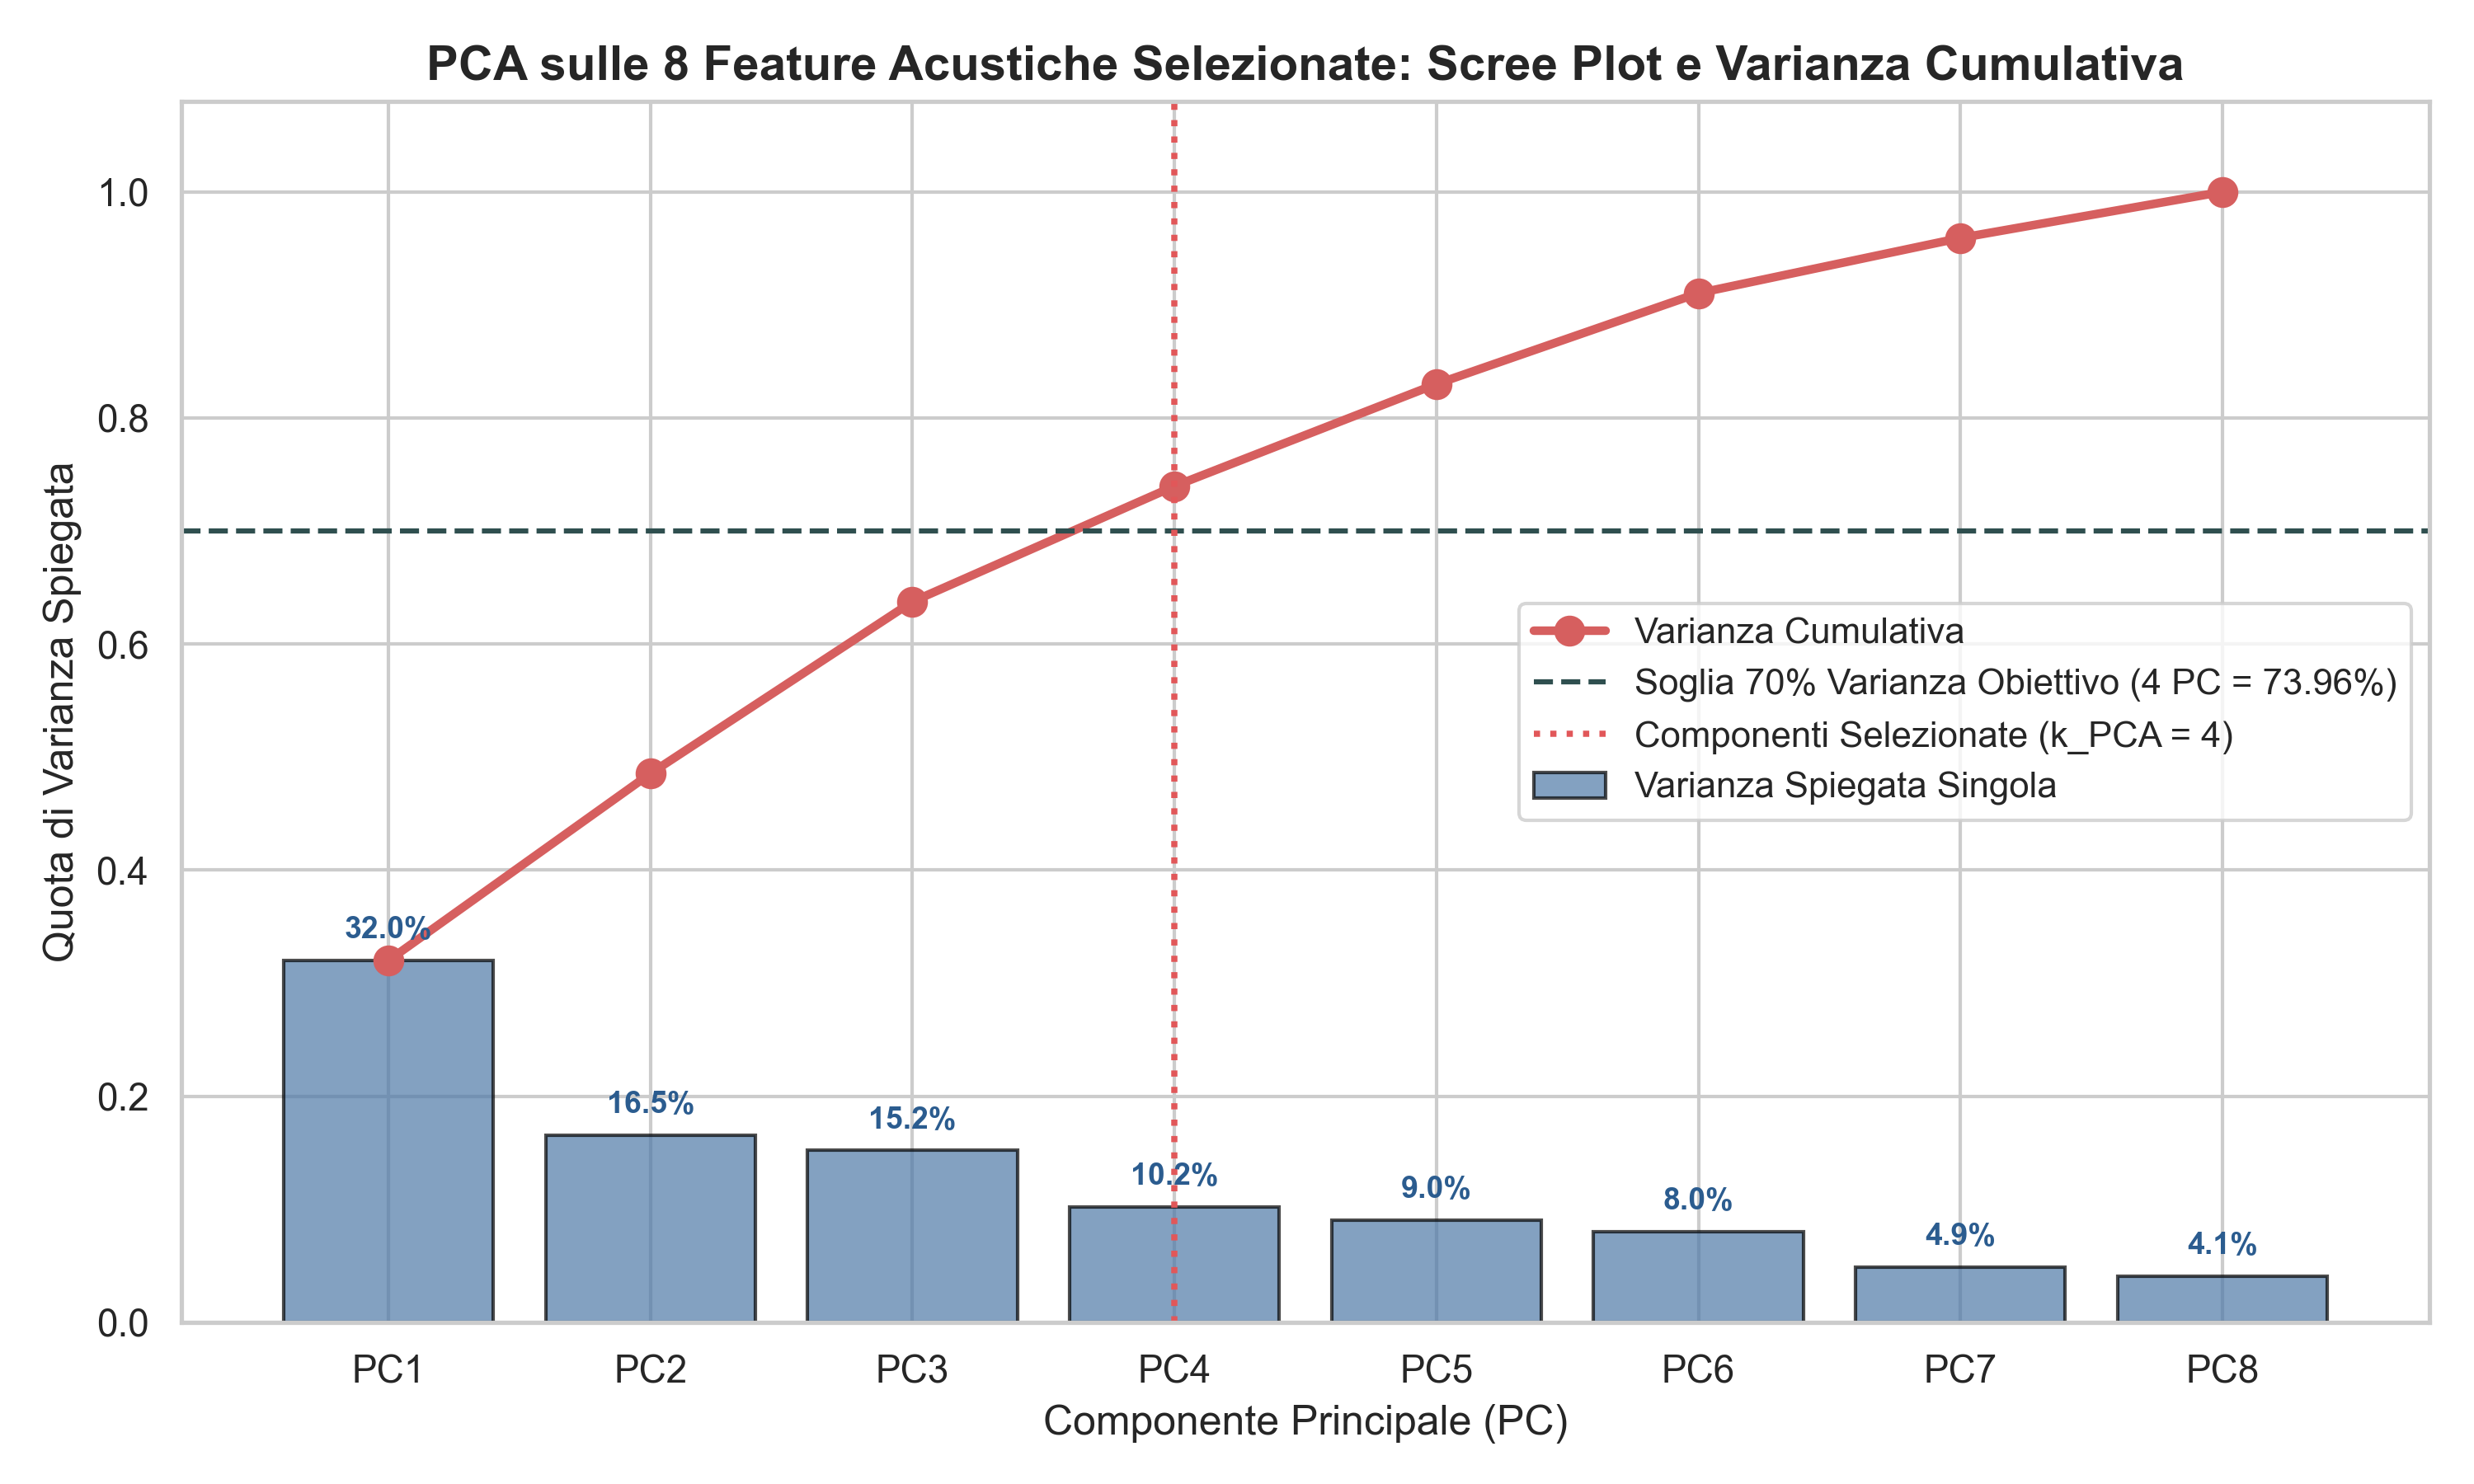
\includegraphics[width=0.78\textwidth]{capitolo4/img/fig14_pca_varianza_cumulativa.png}
    \caption{PCA sulle 8 feature acustiche: Scree Plot della varianza spiegata individuale e cumulativa con soglia obiettivo del 70\%.}
    \label{fig:pca_scree}
\end{figure}

Adottando il criterio della varianza cumulativa minima del 70\%, è stato scelto un numero di componenti pari a \textbf{$\text{n\_components} = 4$}, che preserva il \textbf{73,96\% della varianza totale} e dimezza la dimensionalità dello spazio (da 8 a 4 variabili latenti ortogonali). Il 26,04\% residuo non viene assunto automaticamente come rumore privo di informazione. K-Means, GMM, DBSCAN e HDBSCAN sono confrontati sulla matrice PCA a quattro dimensioni; t-SNE resta una tecnica di visualizzazione.

Ciascuna Componente Principale $\text{PC}_k$ ($k \in \{1, 2, 3, 4\}$) costituisce una nuova "super-variabile" latente ortogonale, ottenuta come combinazione lineare delle 8 feature standardizzate $z_{i,j}$ pesate attraverso i rispettivi coefficienti (\textit{PCA Loadings} $w_{j,k}$):
\begin{equation}
\boxed{\text{PC}_{i,k} = \sum_{j=1}^{8} w_{j,k} \, z_{i,j} = w_{1,k}\, z_{i,\text{dance}} + w_{2,k}\, z_{i,\text{energy}} + \dots + w_{8,k}\, z_{i,\text{duration}}}
\label{eq:pca_linear_comb}
\end{equation}
Per interpretare il significato fisico e musicale dei 4 assi latenti estratti, la Tabella \ref{tab:pca_loadings} riporta la matrice completa dei pesi $w_{j,k}$ che legano le 8 feature originarie alle prime 4 Componenti Principali.

\begin{table}[H]
\centering
\caption{Matrice dei Loadings (pesi lineari) delle prime 4 Componenti Principali rispetto alle 8 feature acustiche standardizzate.}
\label{tab:pca_loadings}
\vspace{0.2cm}
\begin{tabular}{lcccc}
\toprule
\textbf{Feature Acustica} & $\mathbf{PC_1}$ \textbf{(32,00\%)} & $\mathbf{PC_2}$ \textbf{(16,54\%)} & $\mathbf{PC_3}$ \textbf{(15,21\%)} & $\mathbf{PC_4}$ \textbf{(10,22\%)} \\
\midrule
\texttt{danceability}     & $-0,2179$ & $\mathbf{+0,6721}$ & $+0,2303$ & $+0,1679$ \\
\texttt{energy}           & $\mathbf{+0,3767}$ & $-0,2699$ & $\mathbf{+0,5122}$ & $-0,1522$ \\
\texttt{speechiness}      & $\mathbf{-0,3724}$ & $-0,0696$ & $+0,2895$ & $-0,0380$ \\
\texttt{acousticness}     & $\mathbf{-0,3482}$ & $+0,0925$ & $\mathbf{-0,5224}$ & $+0,2265$ \\
\texttt{instrumentalness} & $\mathbf{+0,4838}$ & $+0,2391$ & $-0,0819$ & $+0,3038$ \\
\texttt{valence}          & $-0,2888$ & $+0,2422$ & $\mathbf{+0,5533}$ & $+0,1739$ \\
\texttt{tempo}            & $-0,1770$ & $\mathbf{-0,5300}$ & $+0,1223$ & $\mathbf{+0,7626}$ \\
\texttt{duration\_ms}     & $\mathbf{+0,4494}$ & $+0,2555$ & $+0,0092$ & $\mathbf{+0,4380}$ \\
\bottomrule
\end{tabular}
\end{table}

Dall'ispezione dei coefficienti in Tabella \ref{tab:pca_loadings} emerge una chiara lettura semantica delle 4 dimensioni latenti:
\begin{itemize}
    \item $\mathbf{PC_1}$ \textbf{(32,00\% — Asse Strumentale/Elettronico Esteso vs. Vocale/Acustico Breve):} Presenta pesi positivi marcati su \texttt{instrumentalness} ($+0,4838$), \texttt{duration\_ms} ($+0,4494$) ed \texttt{energy} ($+0,3767$), contrapposti a pesi negativi su \texttt{speechiness} ($-0,3724$) e \texttt{acousticness} ($-0,3482$). Separa nettamente le lunghe tracce elettroniche da club prive di voce dalle canzoni brevi cantate o rappate.
    \item $\mathbf{PC_2}$ \textbf{(16,54\% — Asse Groove Ballabile Cadenzato vs. Velocità Ritmica):} È dominata positivamente dalla \texttt{danceability} ($+0,6721$) e negativamente dal \texttt{tempo} ($-0,5300$) e dall'\texttt{energy} ($-0,2699$). Distingue i brani dal groove cadenzato e ballabile (115--130 BPM) dalle tracce ad altissima velocità di battito e natura frenetica.
    \item $\mathbf{PC_3}$ \textbf{(15,21\% — Asse Euforia Elettrica vs. Intimità Acustica):} Combina contributi positivi elevati di \texttt{valence} ($+0,5533$) ed \texttt{energy} ($+0,5122$) con un forte contributo negativo di \texttt{acousticness} ($-0,5224$), discriminando i brani solari ed energici dalle ballate acustiche ed introspettive.
    \item $\mathbf{PC_4}$ \textbf{(10,22\% — Asse Velocità di Esecuzione e Durata):} È governata prevalentemente dal \texttt{tempo} ($+0,7626$) e da \texttt{duration\_ms} ($+0,4380$), isolando le variazioni puramente metriche e di velocità in BPM.
\end{itemize}

\newpage
\paragraph{t-SNE (t-Distributed Stochastic Neighbor Embedding):}
Accanto alla riduzione lineare PCA (usata per il calcolo effettivo dei cluster), è stata impiegata la tecnica non lineare t-SNE esclusivamente a scopo di visualizzazione topologica bidimensionale su un campione casuale rappresentativo di $N = 6.000$ brani (\texttt{n\_components=2}, \texttt{perplexity=40}, \texttt{random\_state=42}). La Figura \ref{fig:tsne_overview} mostra la mappa t-SNE colorata retrospettivamente con i 15 generi ufficiali di Spotify.

\begin{figure}[H]
    \centering
    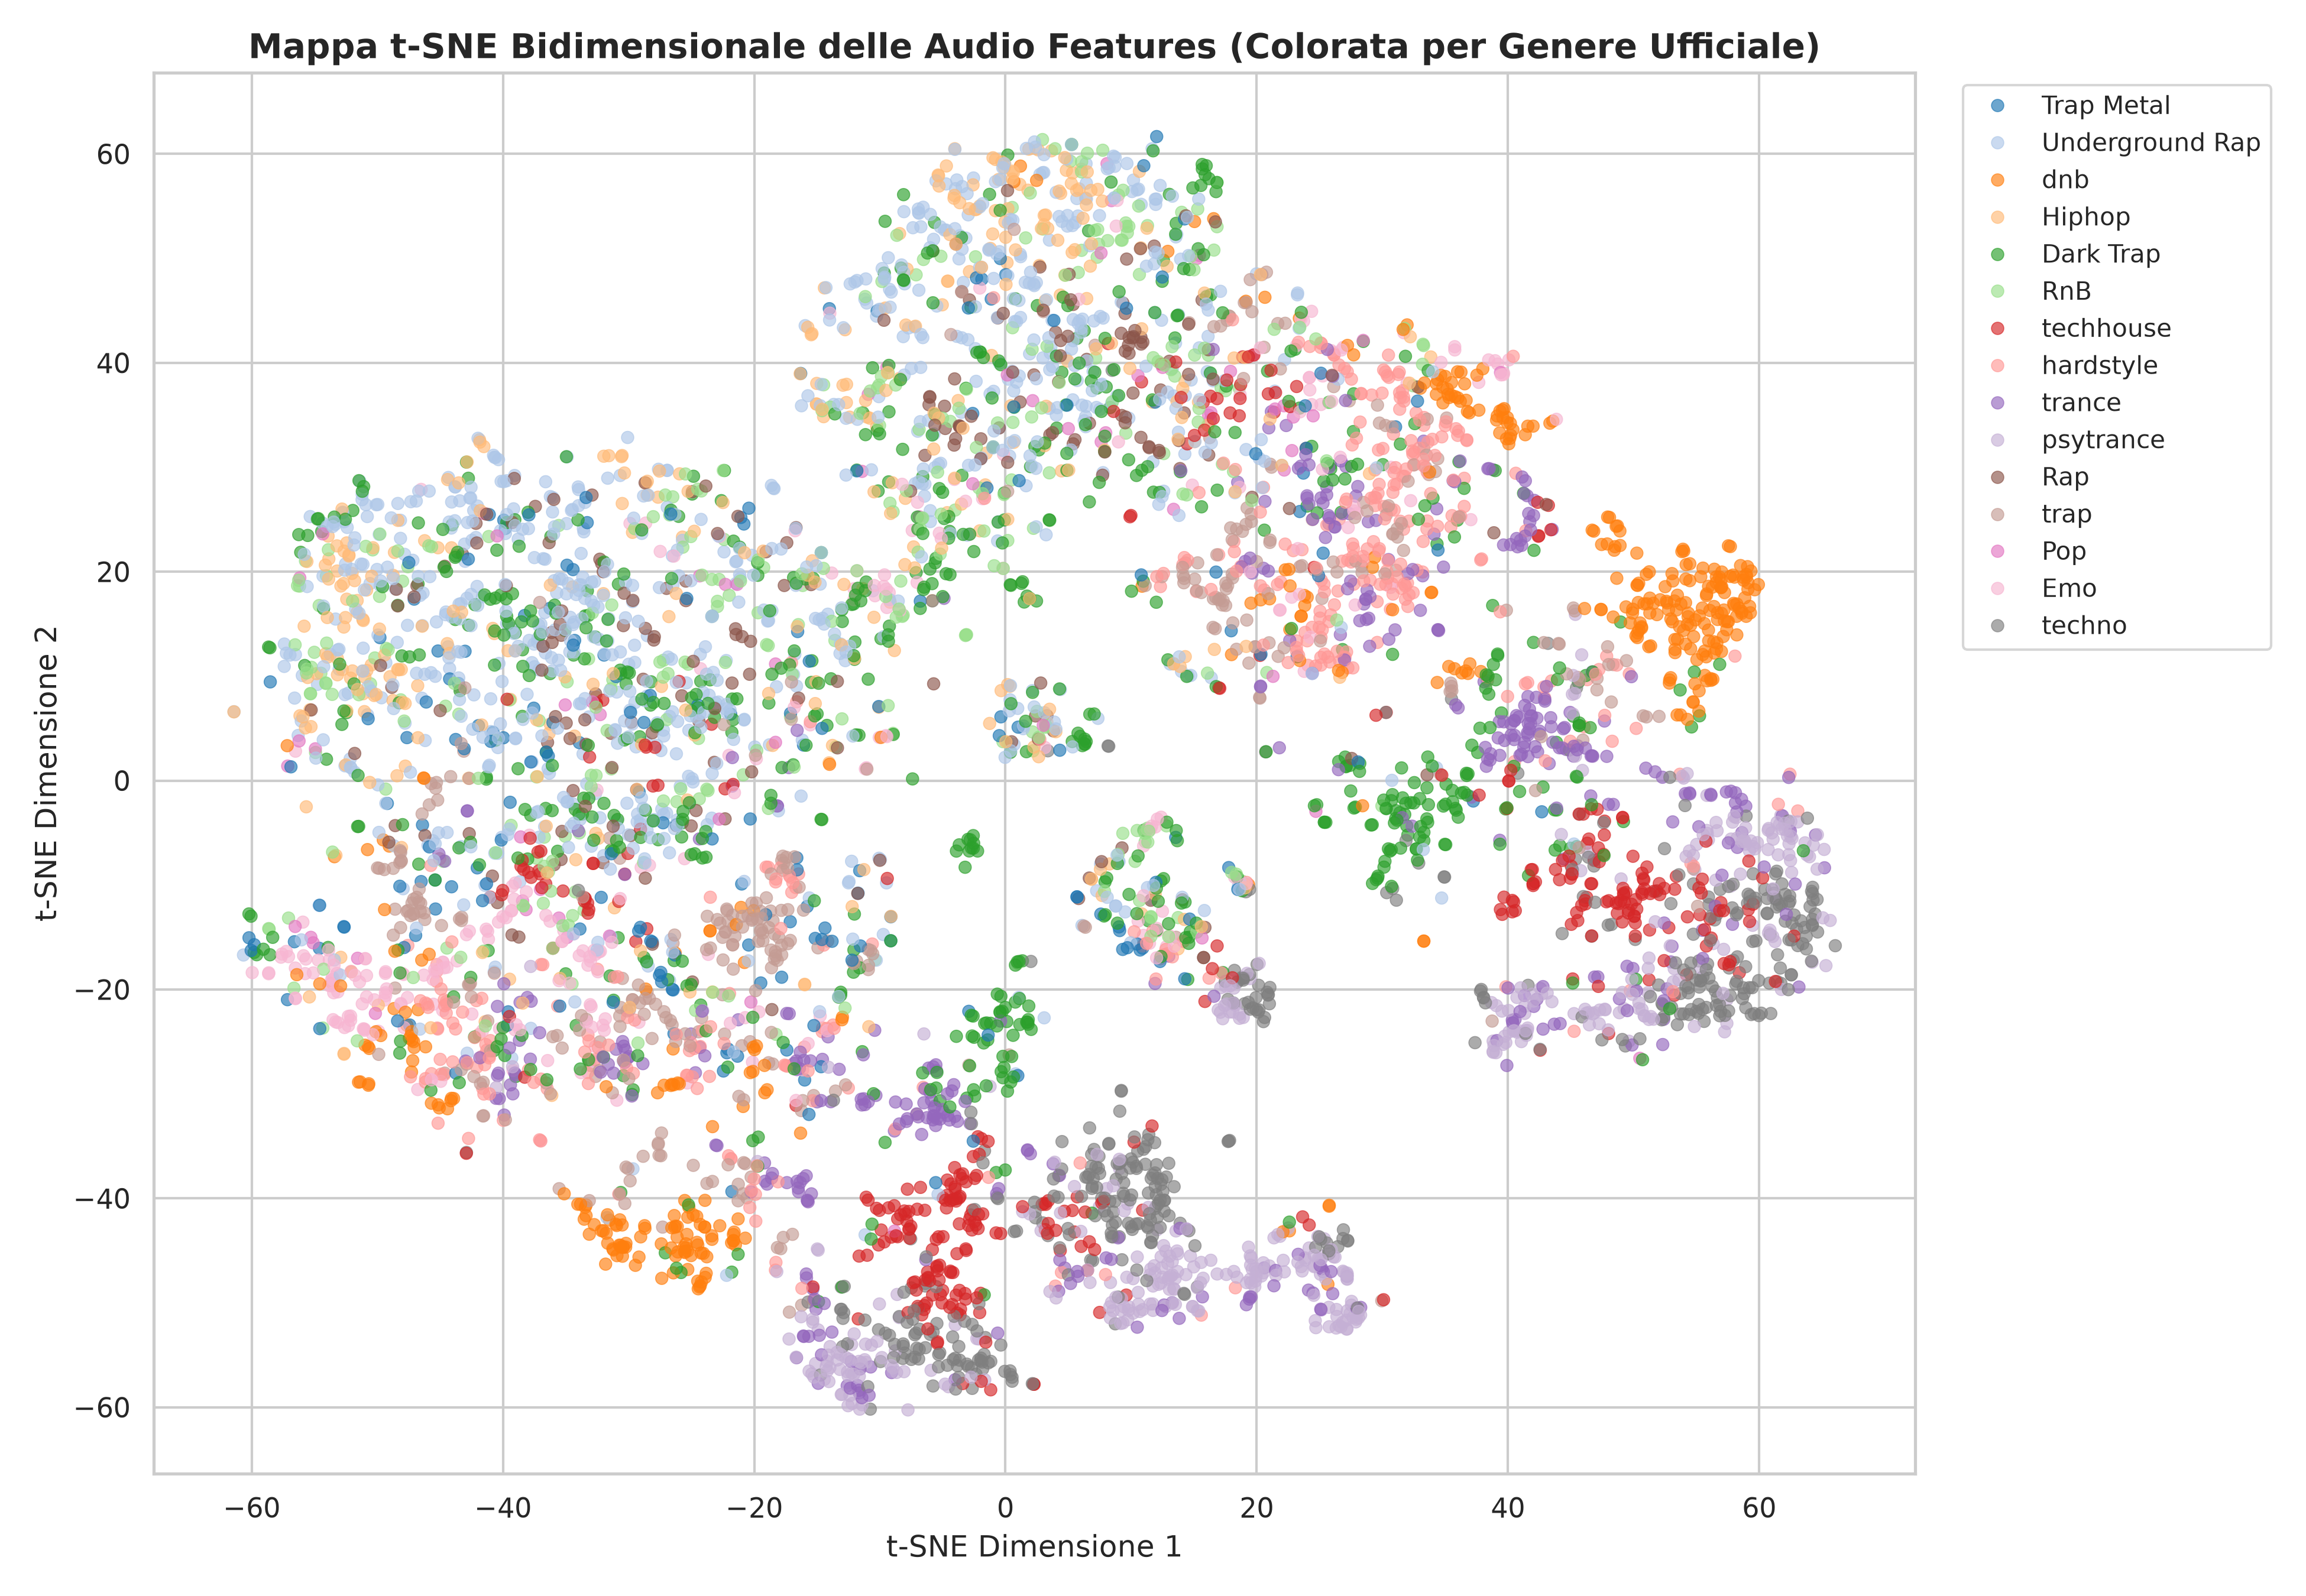
\includegraphics[width=0.86\textwidth]{capitolo4/img/fig15_tsne_2d_overview.png}
    \caption{Mappa 2D generata tramite t-SNE sulle feature acustiche, colorata retrospettivamente per genere Spotify originale.}
    \label{fig:tsne_overview}
\end{figure}

\newpage
\subsection{K-Means nello Spazio PCA}

Il metodo K-Means è un algoritmo di clustering per partizionamento che suddivide le $N$ osservazioni rappresentate nello spazio PCA a 4 dimensioni in $k$ cluster disgiunti $C_1, \dots, C_k$, minimizzando iterativamente la somma dei quadrati delle distanze euclidee intra-cluster (Within-Cluster Sum of Squares, WCSS):
\begin{equation}
\text{WCSS} = \sum_{j=1}^k \sum_{\mathbf{z}_i \in C_j} \|\mathbf{z}_i - \boldsymbol{\mu}_j\|^2
\label{eq:wcss}
\end{equation}
dove $\mathbf{z}_i \in \mathbb{R}^4$ è il vettore delle prime 4 componenti principali del brano $i$-esimo e $\boldsymbol{\mu}_j \in \mathbb{R}^4$ rappresenta il centroide del cluster $C_j$.

\subsubsection{Applicazione dell'algoritmo, Elbow Method e Coefficiente di Silhouette}

Per determinare in modo rigoroso il numero ottimale di cluster $k$ nello spazio PCA a 4 componenti, l'algoritmo K-Means (\texttt{n\_init=20}, \texttt{max\_iter=300}, \texttt{random\_state=42}) è stato valutato per $k \in \{2, 3, \dots, 10\}$ affiancando all'ispezione della curva d'inerzia WCSS (\textit{Elbow Method}) il calcolo del \textbf{Coefficiente di Silhouette medio}, come mostrato nel doppio grafico di Figura \ref{fig:kmeans_elbow}.

\begin{figure}[H]
    \centering
    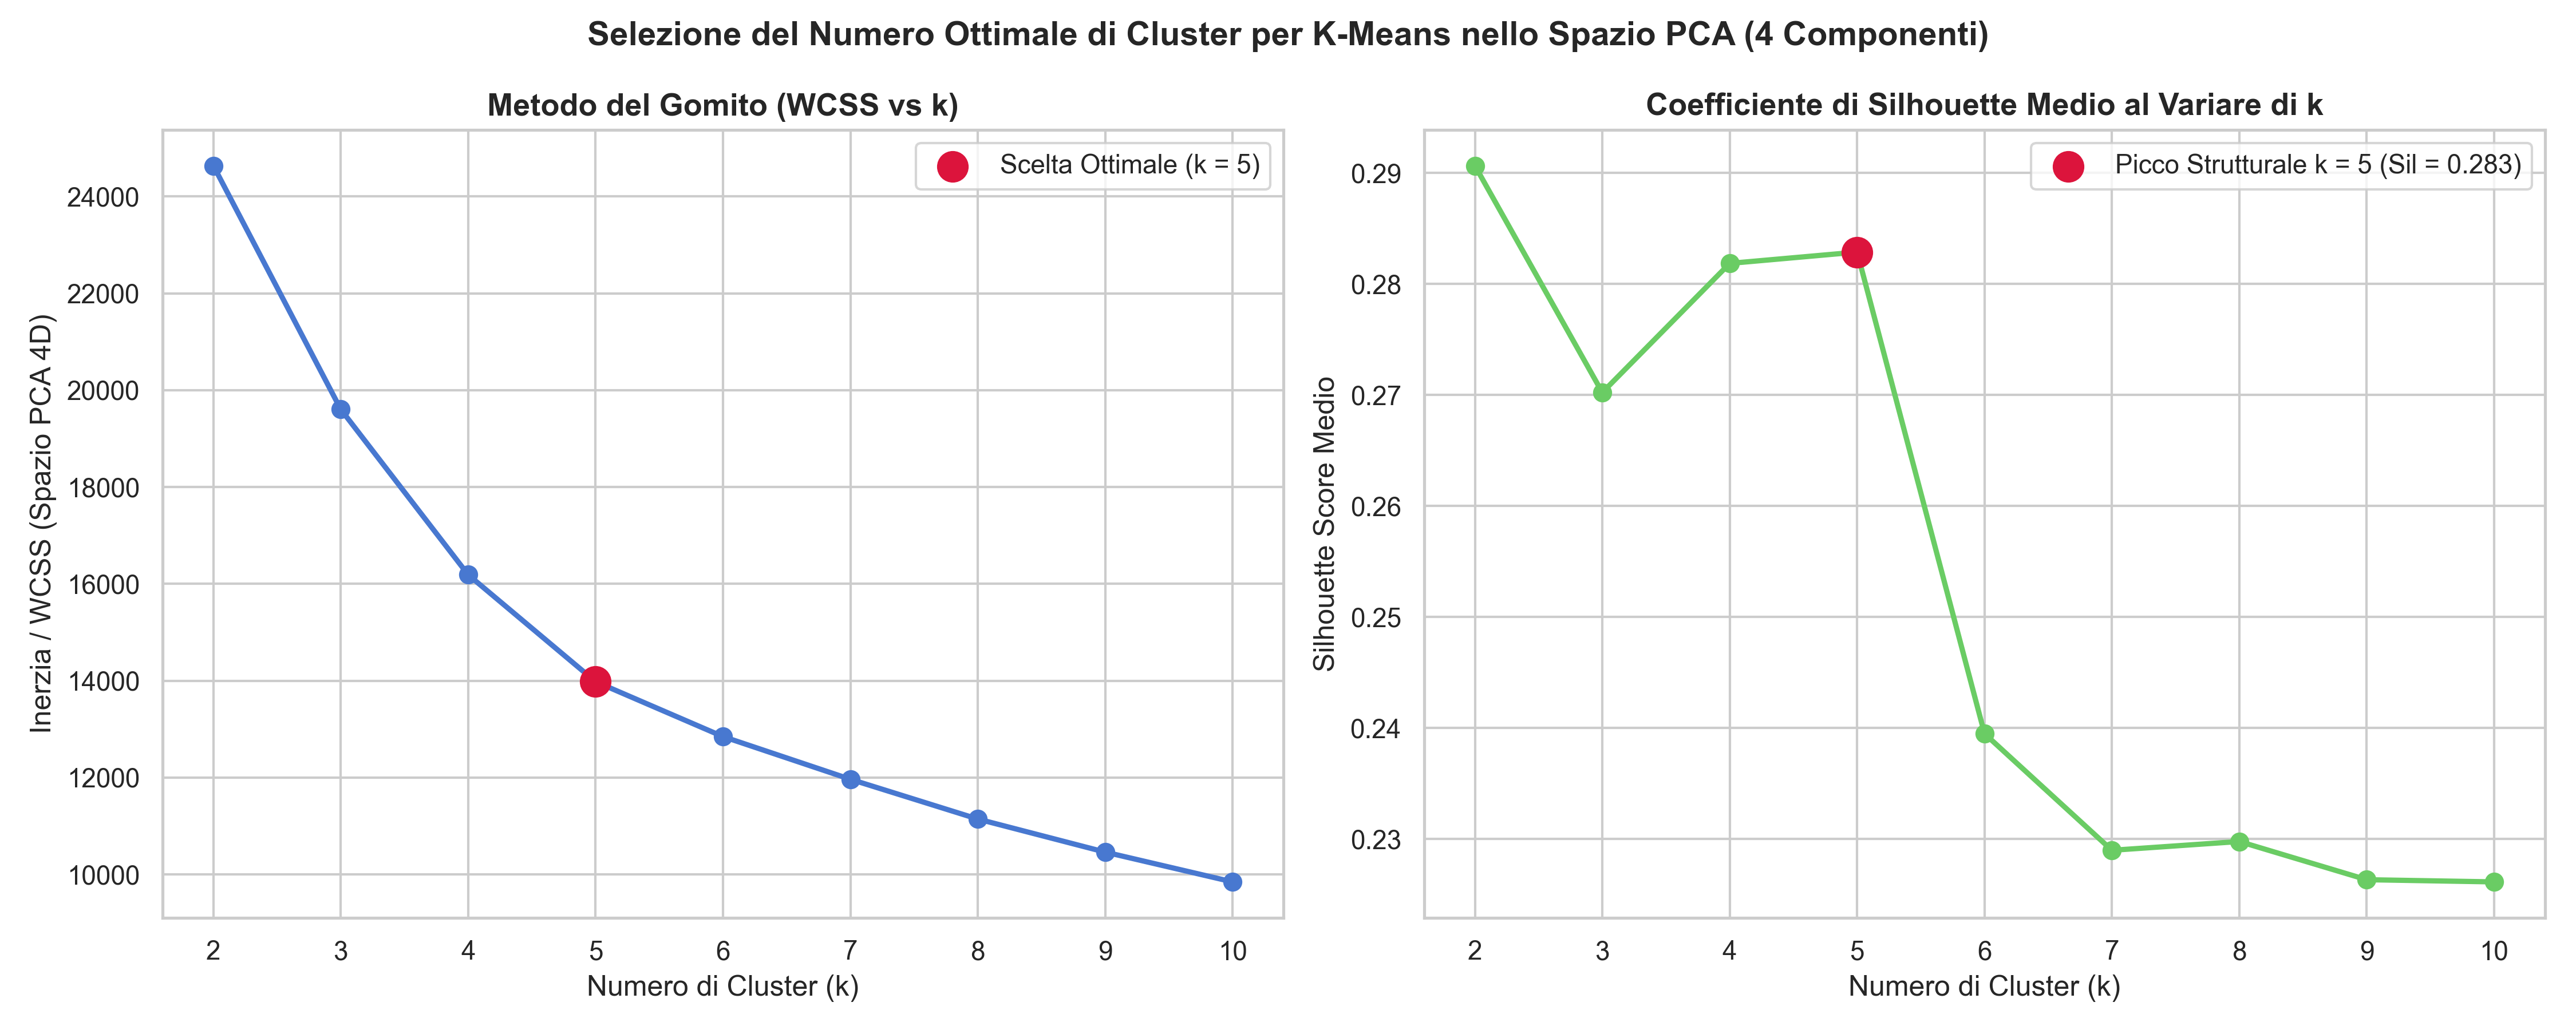
\includegraphics[width=0.95\textwidth]{capitolo4/img/fig16_kmeans_elbow_wcss.png}
    \caption{Selezione del parametro $k$ per K-Means nello spazio PCA (4 PC): curva WCSS (a sinistra) e Coefficiente di Silhouette medio (a destra).}
    \label{fig:kmeans_elbow}
\end{figure}

L'analisi congiunta dei due indicatori in Figura \ref{fig:kmeans_elbow} fornisce una giustificazione matematica univoca per la scelta di \textbf{$k = 5$}:
\begin{enumerate}
    \item Sulla curva WCSS (pannello sinistro), la pendenza subisce una netta decelerazione dopo $k = 5$ ($\text{WCSS} = 13.981,8$), punto oltre il quale l'aggiunta di ulteriori centroidi produce riduzioni marginali dell'inerzia intra-cluster.
    \item Sulla curva della Silhouette media (pannello destro), dopo i valori registrati a $k=3$ ($0,2702$) e $k=4$ ($0,2819$), la compattezza raggiunge un \textbf{massimo locale strutturale esattamente in corrispondenza di $k = 5$ con $\text{Silhouette} = 0,2829$}, prima di subire un brusco calo a $k = 6$ ($\text{Silhouette} = 0,2395$) dovuto alla frammentazione artificiale dei gruppi principali.
\end{enumerate}

\subsubsection{Analisi dei risultati ottenuti e proiezioni spaziali}

Il modello K-Means addestrato con $k = 5$ sulle 4 componenti principali ha generato una partizione bilanciata e ben strutturata sia sul campione di analisi ($N = 6.000$) sia sull'intero catalogo deduplicato ($N = 35.877$), come riepilogato nella Tabella \ref{tab:kmeans_counts}.

\begin{table}[H]
\centering
\caption{Distribuzione numerica e percentuale dei brani nei 5 cluster K-Means (campione di analisi e intero catalogo deduplicato).}
\label{tab:kmeans_counts}
\vspace{0.2cm}
\resizebox{\textwidth}{!}{%
\begin{tabular}{llccc}
\toprule
\textbf{Cluster} & \textbf{Archetipo Musicale (Mood Playlist)} & \textbf{Campione ($N=6.000$)} & \textbf{Catalogo ($N=35.877$)} & \textbf{Quota (\%)} \\
\midrule
\textbf{Cluster 0} & High-Intensity Bass \& Workout        & 1.710 & 10.583 & 29,50\% \\
\textbf{Cluster 1} & Extended Club \& Instrumental         & 1.517 & 8.964  & 24,99\% \\
\textbf{Cluster 2} & Acoustic, Chill \& Atmospheric        & 549   & 3.189  & 8,89\%  \\
\textbf{Cluster 3} & Groove, Melodic Urban \& Dance-Pop    & 1.250 & 7.354  & 20,50\% \\
\textbf{Cluster 4} & Fast-Flow Rap \& High-Tempo Urban     & 974   & 5.787  & 16,13\% \\
\bottomrule
\end{tabular}}
\end{table}

La Figura \ref{fig:kmeans_tsne} illustra la disposizione geometrica dei 5 cluster affiancando la proiezione lineare nel piano delle prime due componenti principali ($\text{PC}_1$ vs $\text{PC}_2$, con indicazione esplicita dei 5 centroidi $\mathbf{X}$) e la proiezione non lineare sulla mappa t-SNE.

\begin{figure}[H]
    \centering
    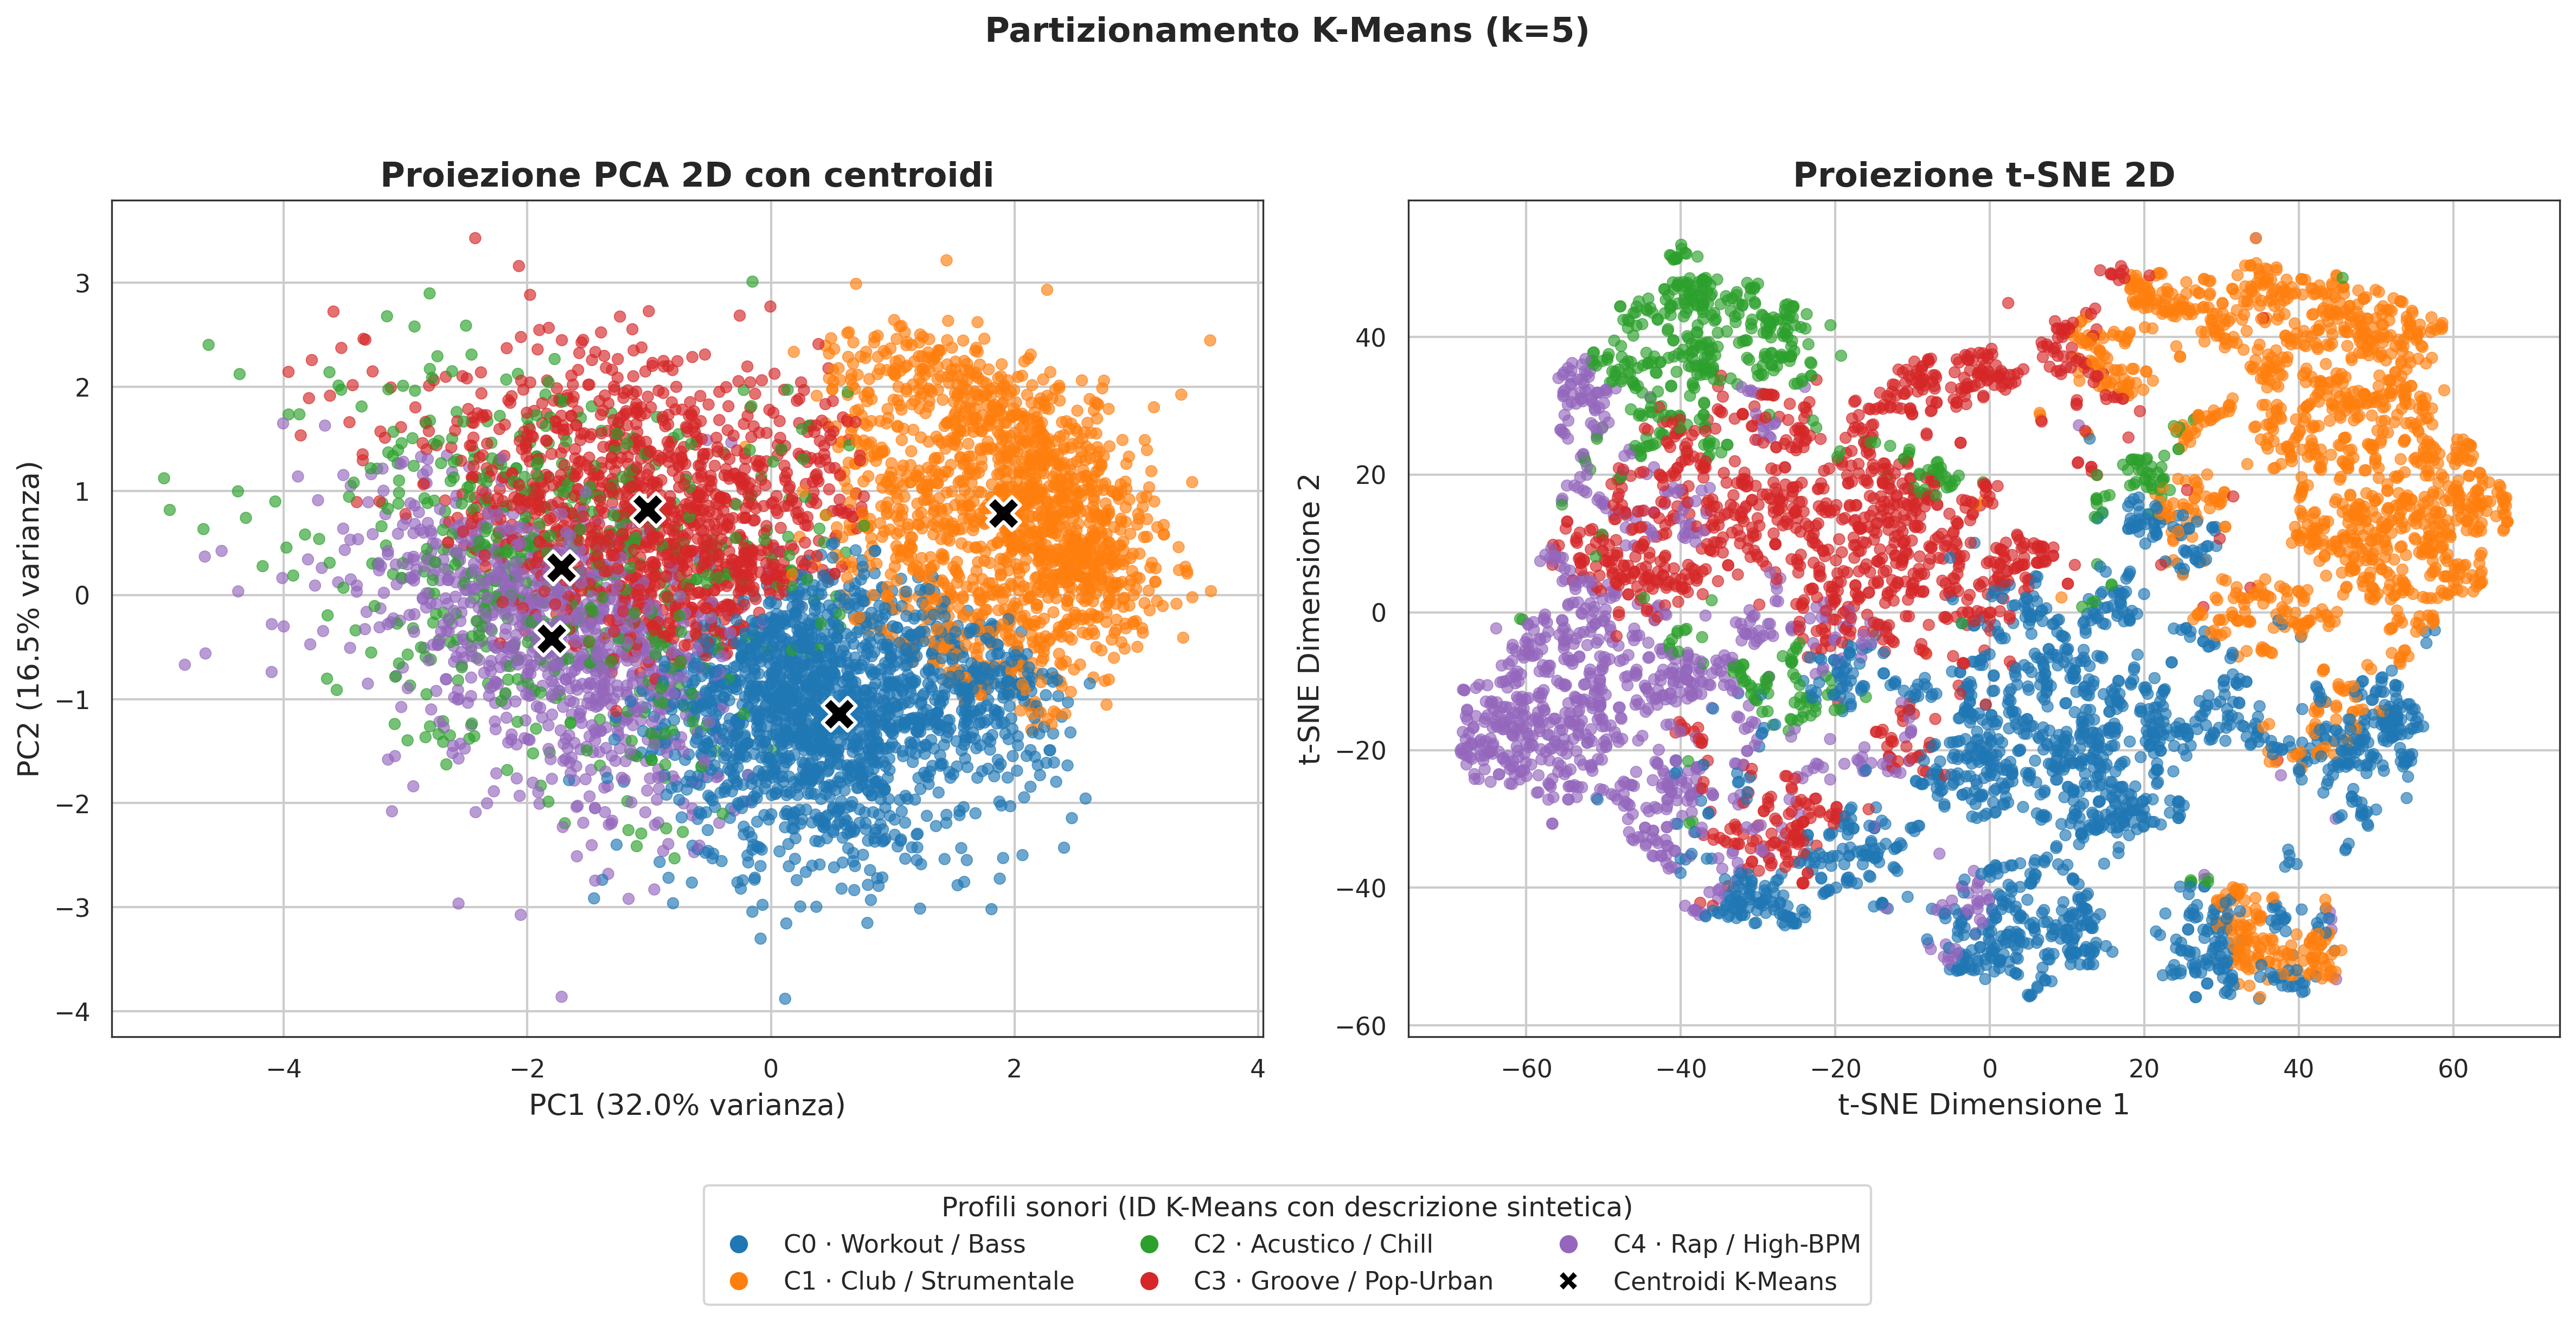
\includegraphics[width=0.98\textwidth]{capitolo4/img/fig17_kmeans_tsne_clusters.png}
    \caption{Partizionamento K-Means ($k=5$) visualizzato nel piano lineare PCA ($\text{PC}_1$ vs $\text{PC}_2$ con centroidi) e sulla mappa non lineare t-SNE 2D.}
    \label{fig:kmeans_tsne}
\end{figure}

Dalla Figura \ref{fig:kmeans_tsne} si osserva come nel piano PCA i 5 centroidi presidino regioni ben distinte dello spazio delle componenti principali, e come tale partizione si traduca, sulla varietà non lineare t-SNE, in macro-regioni timbriche coerenti e prive di sovrapposizioni caotiche.

\newpage
\subsubsection{Profiling acustico dei Cluster e Mood Playlists}

Per interpretare il significato musicale e funzionale dei 5 cluster, la Figura \ref{fig:kmeans_profile_heatmap} riporta una heatmap delle medie osservate. Le annotazioni contengono i valori medi originali (la durata è espressa in migliaia di millisecondi), mentre il colore è normalizzato Min-Max separatamente per ciascuna feature: il colore consente quindi di confrontare i cluster sulla stessa variabile, non grandezze assolute tra variabili diverse. La matrice include anche \texttt{loudness} e \texttt{liveness} come descrittori retrospettivi; queste due variabili non sono state usate per addestrare K-Means né per costruire lo spazio PCA.

\begin{figure}[H]
    \centering
    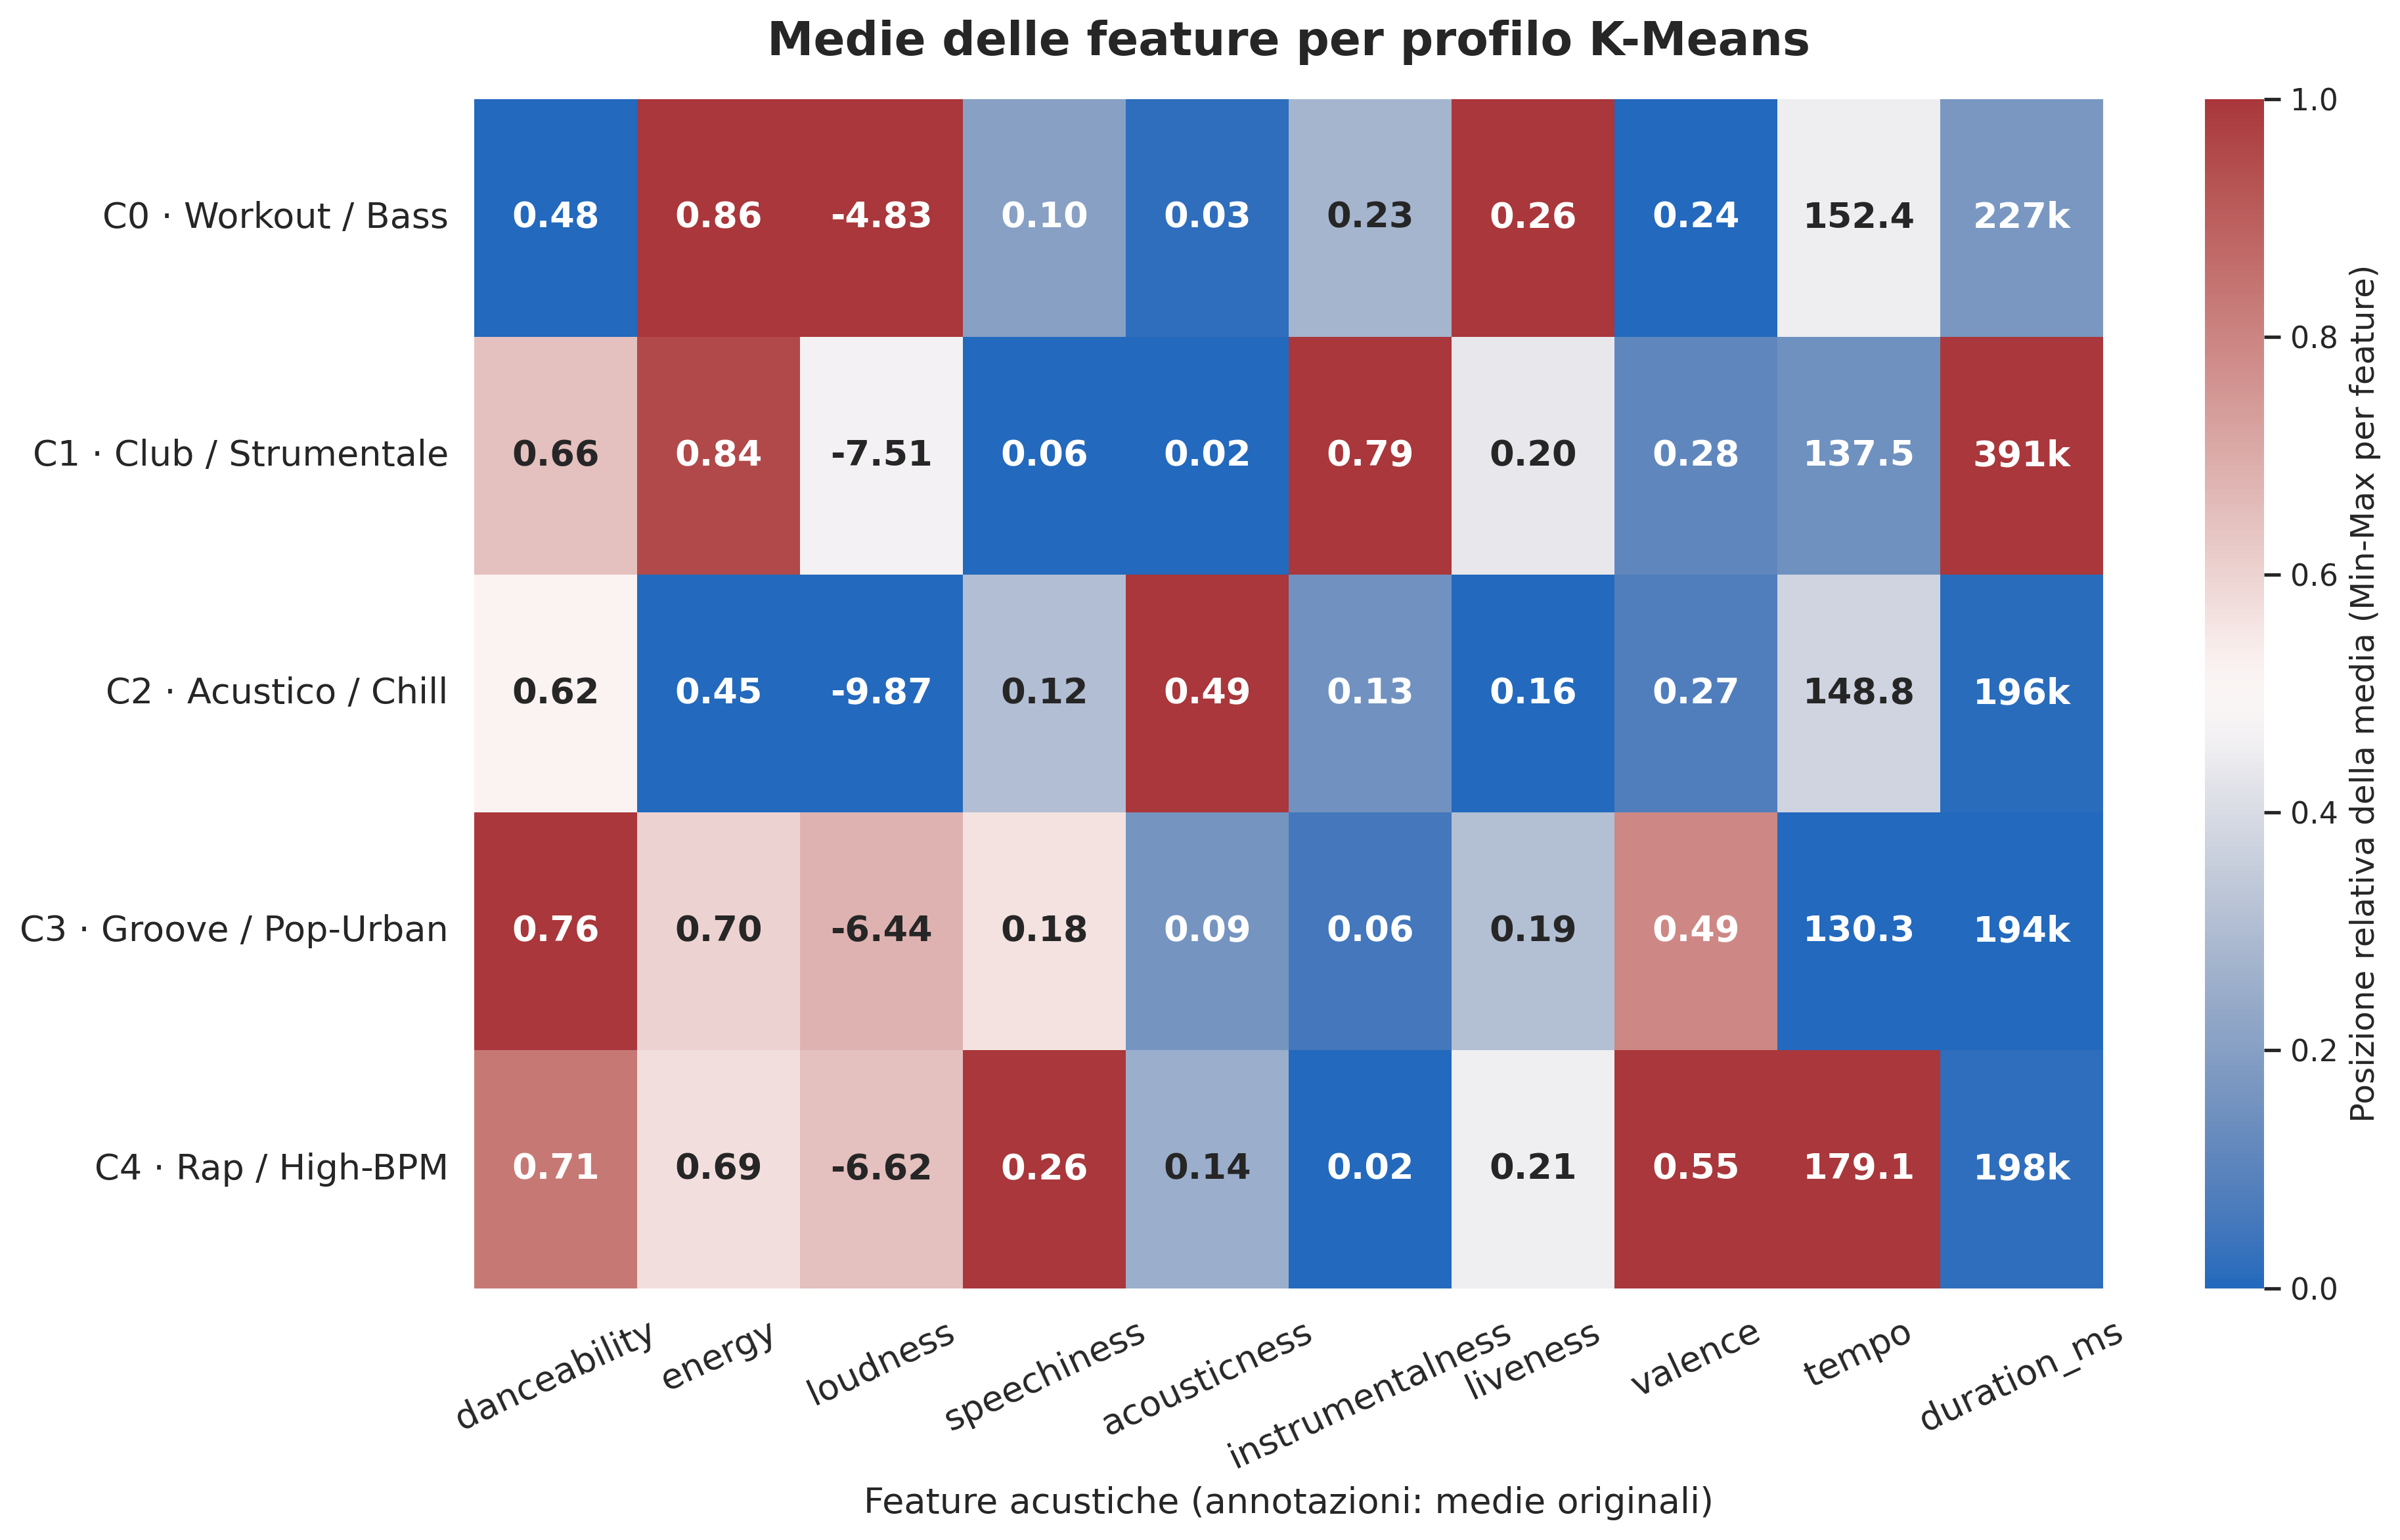
\includegraphics[width=\textwidth]{capitolo4/img/fig18_kmeans_feature_profiling.png}
    \caption{Medie delle feature per i cluster K-Means. Le annotazioni riportano le medie originali; il colore è riscalato per colonna.}
    \label{fig:kmeans_profile_heatmap}
\end{figure}

La matrice mette in evidenza differenze utili a descrivere i profili: C1 presenta una forte strumentalità e durate maggiori; C2 ha maggiore acusticità e minore energia; C3 è il profilo più ballabile, mentre C4 mostra tempo e contenuto parlato più elevati. C0 combina energia e volume mediamente alti. Le sigle C0--C4 sono identificativi; i nomi brevi riportati in legenda riassumono i tratti dominanti, senza essere etichette di genere.

La Figura \ref{fig:kmeans_profile_radar} visualizza in forma polare gli stessi profili limitandosi alle 8 feature effettivamente usate nel clustering. Anche in questo grafico ciascun asse è normalizzato tra i cluster: la forma rende immediato il confronto relativo tra profili, ma non va letta come confronto delle unità originali o come intensità assoluta della feature.

\begin{figure}[H]
    \centering
    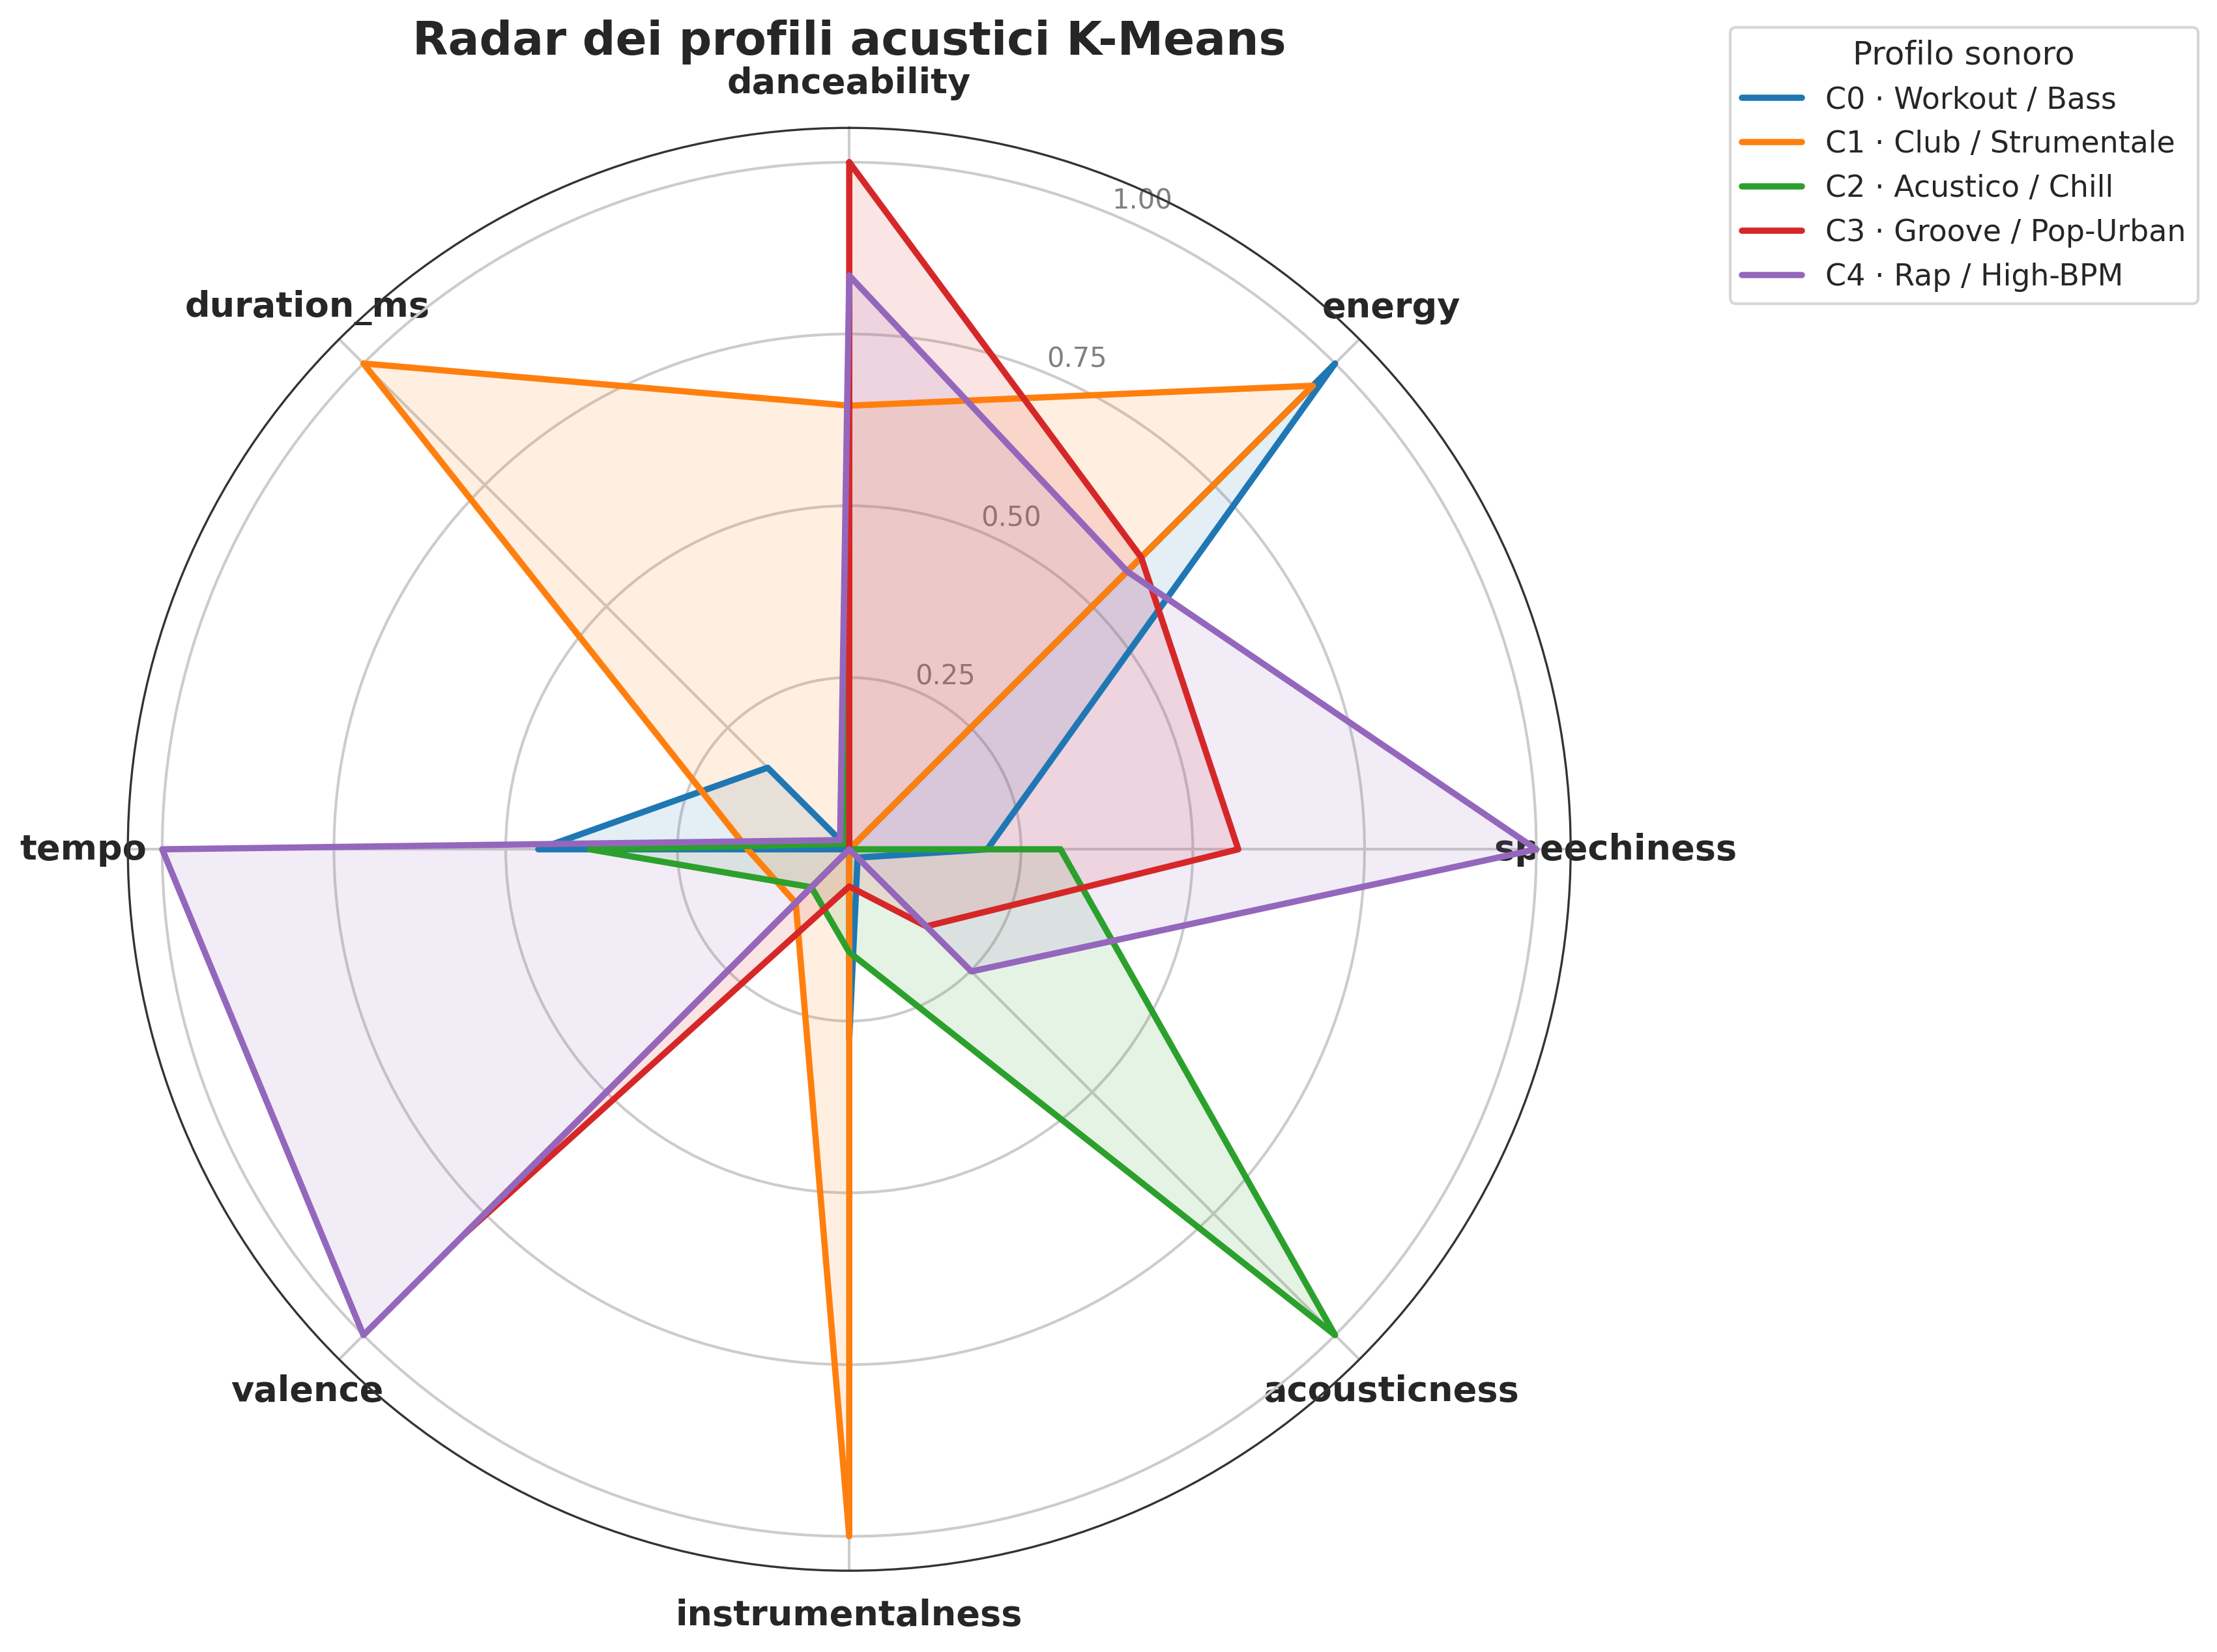
\includegraphics[width=0.98\textwidth]{capitolo4/img/fig19_kmeans_feature_radar.png}
    \caption{Radar chart delle medie normalizzate delle 8 feature usate nel clustering K-Means.}
    \label{fig:kmeans_profile_radar}
\end{figure}

Dall'esame congiunto delle Figure \ref{fig:kmeans_profile_heatmap} e \ref{fig:kmeans_profile_radar}, oltre che dall'incrocio retrospettivo con i generi originali, ciascun cluster rivela un'identità acustica e funzionale netta:
\begin{itemize}
    \item \textbf{Cluster 0 — High-Intensity Bass \& Workout ($1.710$ brani campione / $10.583$ catalogo):} È il cluster a massima potenza d'urto: registra i valori medi più elevati in assoluto di \texttt{energy} ($0,86$) e \texttt{loudness} ($-4,83\text{ dB}$), uniti a un \texttt{tempo} sostenuto ($152,40\text{ BPM}$), ma con la più bassa \texttt{danceability} ($0,48$) e una \texttt{valence} scura/aggressiva ($0,24$). Raccoglie in larga misura tracce \textit{Hardstyle}, \textit{Drum and Bass} e \textit{Trap/Trap Metal} ad alto impatto adrenalinico, perfette per playlist di allenamento intenso (\textit{Workout / Gym}).
    \item \textbf{Cluster 1 — Extended Club \& Instrumental Electronic ($1.517$ brani campione / $8.964$ catalogo):} Si distingue in modo inequivocabile per l'altissima \texttt{instrumentalness} media ($0,79$, contro $0,02\text{--}0,23$ degli altri gruppi) e per la durata media estesa (\texttt{duration\_ms} $= 390.803\text{ ms}$, circa $6,5$ minuti), accompagnate da \texttt{energy} elevata ($0,84$), ottima \texttt{danceability} ($0,66$), \texttt{speechiness} minima ($0,06$) e battito regolare da club ($137,52\text{ BPM}$). Cattura i brani \textit{Techno}, \textit{Psytrance}, \textit{Trance} e \textit{Techhouse} pensati per il DJ mixing e per sessioni di \textit{Deep Focus / Clubbing}.
    \item \textbf{Cluster 2 — Acoustic, Chill \& Atmospheric ($549$ brani campione / $3.189$ catalogo):} Rappresenta il polo intimo e decompressivo del catalogo: presenta il valore massimo di \texttt{acousticness} ($0,49$, oltre tre volte superiore a qualsiasi altro cluster) e i livelli minimi di \texttt{energy} ($0,45$) e volume (\texttt{loudness} $= -9,87\text{ dB}$), con durata contenuta ($196.127\text{ ms}$). Raggruppa produzioni acustiche, R\&B morbido, Emo e tracce \textit{Dark Trap / Lo-Fi} rarefatte, ideali per playlist \textit{Chillout, Late Night \& Relax}.
    \item \textbf{Cluster 3 — Groove, Melodic Urban \& Dance-Pop ($1.250$ brani campione / $7.354$ catalogo):} È il cluster a più alta ballabilità dell'intero dataset (\texttt{danceability} $= 0,76$), caratterizzato da un \texttt{tempo} moderato e cadenzato ($130,31\text{ BPM}$), \texttt{valence} positiva ($0,49$), buona \texttt{energy} ($0,70$), presenza vocale ritmica (\texttt{speechiness} $= 0,18$) e quasi totale assenza strumentale ($0,06$). Aggrega in modo trasversale \textit{Pop}, \textit{R\&B}, \textit{Rap melodico} e \textit{Techhouse} radiofonica, costituendo l'archetipo perfetto per playlist \textit{Social Groove \& Aperitif}.
    \item \textbf{Cluster 4 — Fast-Flow Rap \& High-Tempo Urban ($974$ brani campione / $5.787$ catalogo):} Isola i brani caratterizzati dalla massima velocità ritmica (\texttt{tempo} medio $= 179,12\text{ BPM}$), dalla massima densità di parlato/rima (\texttt{speechiness} $= 0,26$) e dalla più alta positività/dinamismo (\texttt{valence} $= 0,55$), con \texttt{danceability} elevata ($0,71$) e durata compatta ($197.699\text{ ms}$). È composto prevalentemente da \textit{Underground Rap}, \textit{Hiphop} e \textit{Dark Trap} in doppia metrica, ideale per playlist \textit{Street Flow \& High-BPM Urban}.
\end{itemize}

\newpage
\subsubsection{Valutazione della Silhouette per K-Means}

Per valutare la coesione interna e la separazione di ciascuno dei 5 gruppi individuati nello spazio PCA a 4 dimensioni, è stato calcolato il coefficiente di Silhouette puntuale $s(i)$ per ogni brano del campione secondo la formula:
\begin{equation}
s(i) = \frac{b(i) - a(i)}{\max(a(i), b(i))}
\label{eq:silhouette}
\end{equation}
dove $a(i)$ è la distanza euclidea media tra il brano $i$ e gli altri brani del medesimo cluster nello spazio PCA 4D, mentre $b(i)$ è la distanza media minima rispetto ai brani del cluster contiguo più vicino. La Figura \ref{fig:kmeans_silhouette} mostra la distribuzione dei coefficienti di Silhouette per i 5 cluster.

\begin{figure}[H]
    \centering
    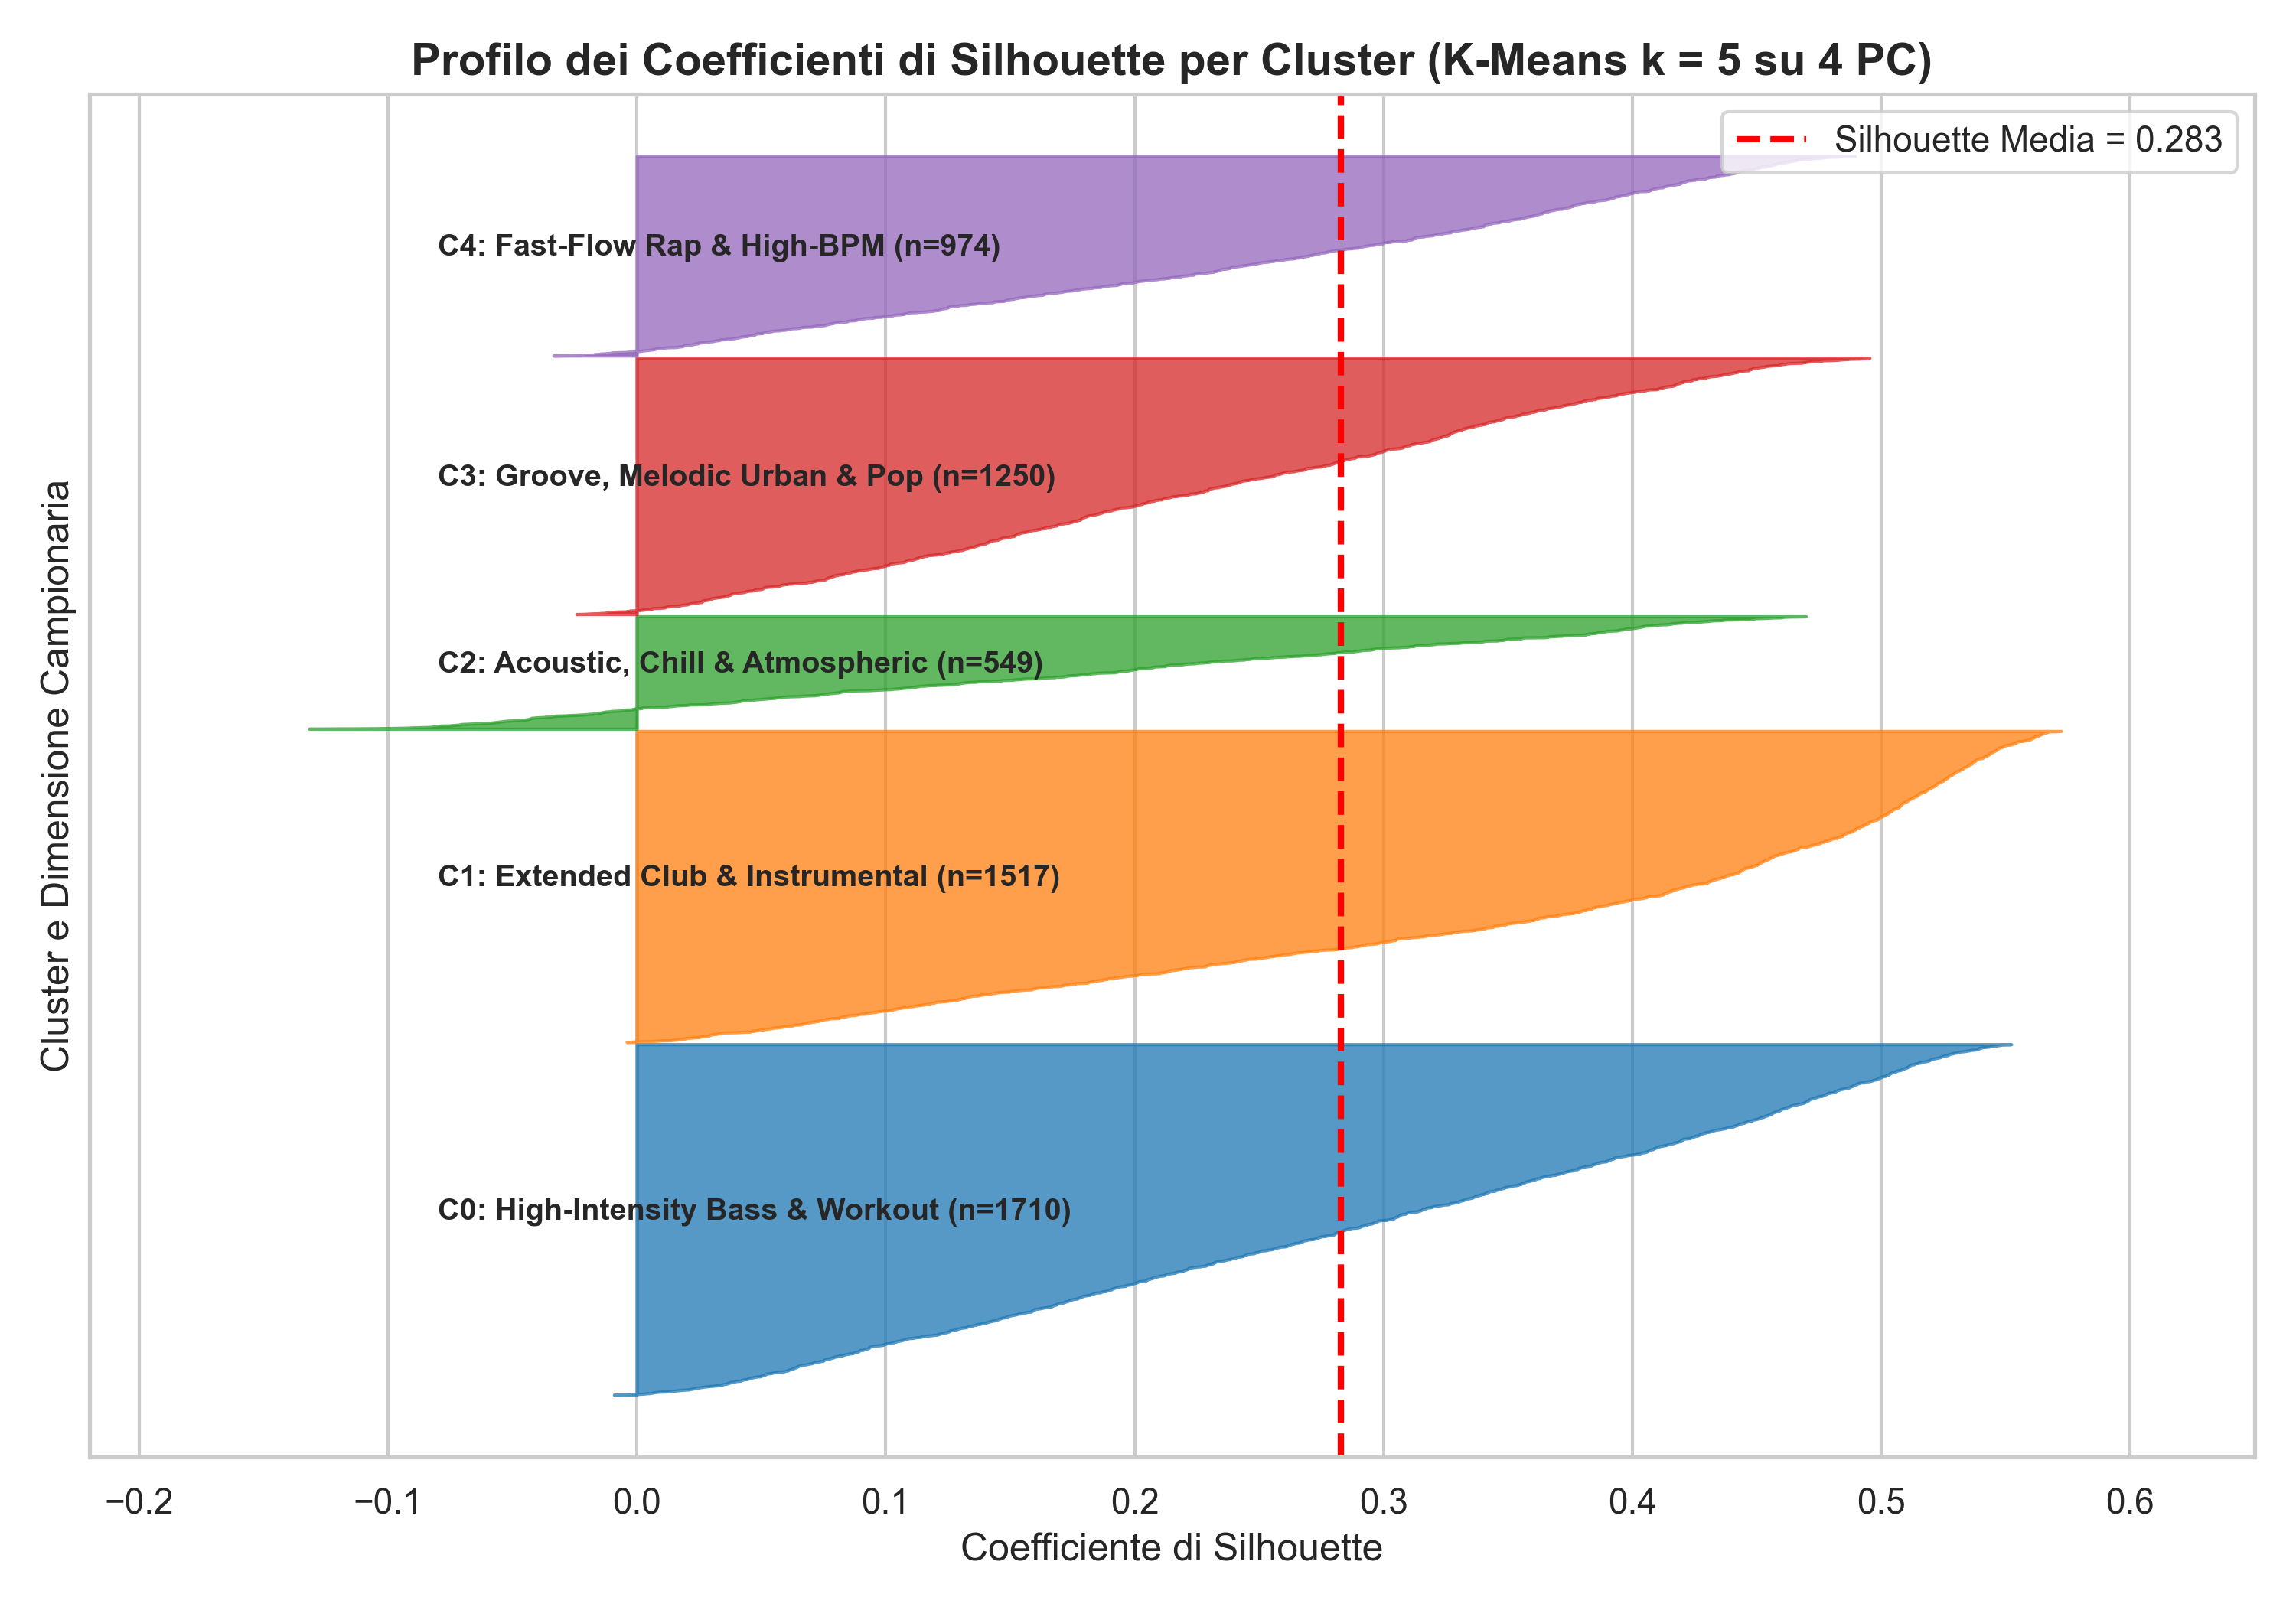
\includegraphics[width=0.78\textwidth]{capitolo4/img/fig19_kmeans_silhouette_plot.png}
    \caption{Profilo dei coefficienti di Silhouette per ciascun cluster K-Means ($k=5$) calcolato nello spazio PCA a 4 componenti.}
    \label{fig:kmeans_silhouette}
\end{figure}

Dalla Figura \ref{fig:kmeans_silhouette} emerge un valore medio globale di Silhouette pari a \textbf{$0,2829$} (notevolmente superiore al valore di $0,1204$ che si otterrebbe applicando K-Means direttamente sulle 13 variabili non ridotte). Tutti e 5 i cluster superano ampiamente la soglia media con picchi superiori a $0,50$ (in particolare il Cluster 1 strumentale e i Cluster 3 e 4 urban/groove) e una frazione molto ridotta di valori negativi (punti di confine). Un valore di Silhouette intorno a $0,28\text{--}0,30$ è pienamente coerente con la natura fisica dei dati musicali: a differenza di dataset sintetici con isole disgiunte, gli attributi acustici formano una varietà continua in cui le transizioni tra stili avvengono gradualmente, e K-Means opera efficacemente una tassonomia geometrica convessa di tale continuum.

\subsubsection{Evoluzione probabilistica di K-Means: Gaussian Mixture Model}
K-Means assegna ciascun brano in modo deterministico e rigido a un solo cluster, anche quando le sue coordinate metriche cadono esattamente nella terra di nessuno tra due o più profili. Nel dominio musicale, tuttavia, i generi e gli stati emotivi formano un continuum sfumato: una traccia \textit{RnB contemporanea} può combinare un groove ritmico ballabile con una timbrica vocale intima ed acustica, rendendo riduttiva l'assegnazione a un singolo contenitore disgiunto. Per superare questa limitazione geometrica e catturare la natura polivalente della musica, è stato introdotto un \textit{Gaussian Mixture Model} (GMM) a cinque componenti con matrice di covarianza piena (\texttt{covariance\_type='full'}), addestrato sul medesimo campione di $N=6.000$ brani nello spazio PCA a 4 dimensioni.

Il modello stima per ogni traccia un vettore di affiliazioni probabilistiche $\boldsymbol{\gamma}_i = (\gamma_{i,0}, \dots, \gamma_{i,4})$, dove $\sum_{k=0}^4 \gamma_{i,k} = 1$. Questi valori quantificano l'appartenenza a ciascuno dei 5 macro-archetipi nello spazio acustico latente. La Figura \ref{fig:gmm_soft} illustra la topografia del modello proiettata sul piano delle prime due componenti principali, evidenziando le ellissi di covarianza a $1\sigma$ (intervallo di confidenza al 68\%) e $2\sigma$ (intervallo al 95\%), unitamente alla classificazione empirica dei corridoi ibridi più popolati.

\begin{figure}[H]
    \centering
    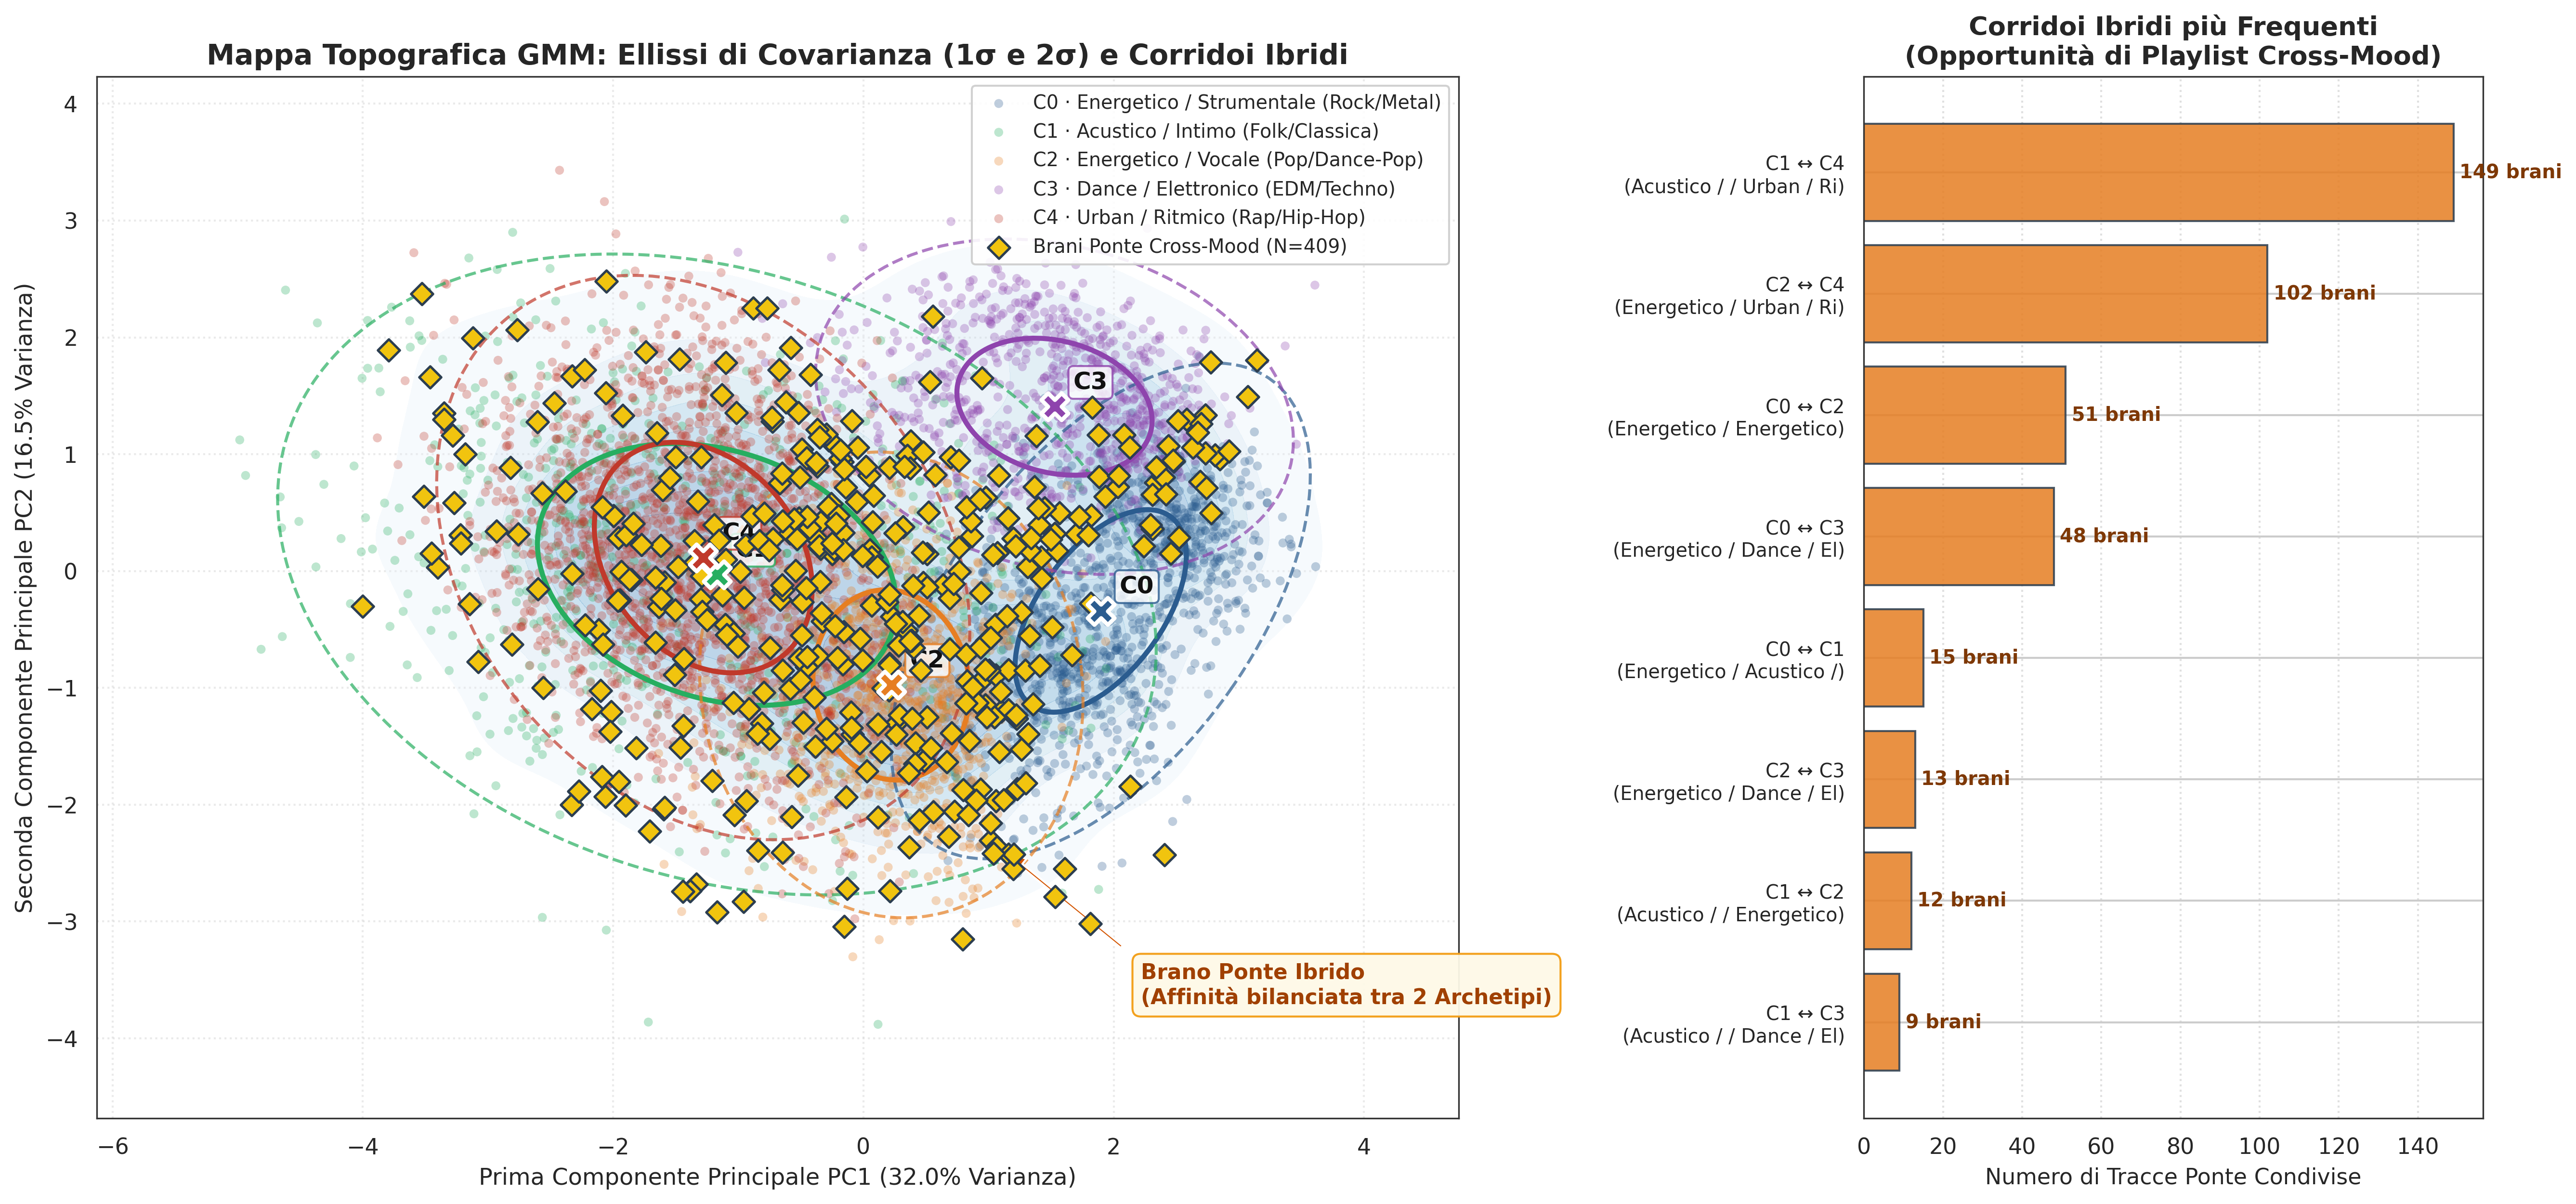
\includegraphics[width=\textwidth]{capitolo4/img/fig24_gmm_soft_membership.png}
    \caption{Mappa topografica GMM nello spazio PCA 2D con ellissi di dispersione ($1\sigma$ continua, $2\sigma$ tratteggiata) ed evidenziazione dei 409 brani ponte cross-mood (a sinistra), affiancata dalla graduatoria dei corridoi ibridi più frequenti (a destra).}
    \label{fig:gmm_soft}
\end{figure}

Per tradurre intuitivamente la complessa interazione probabilistica a 5 dimensioni, la Figura \ref{fig:gmm_radviz} introduce il \textbf{Pentagono Baricentrico dei Mood (RadViz Simplex Plot)}. I 5 vertici del pentagono rappresentano gli archetipi "puri" ($\gamma_{i,k} = 1$); ciascun brano viene posizionato nel piano mediante la combinazione lineare convessa dei vettori dei vertici pesata sulle rispettive probabilità:
\begin{equation}
\mathbf{P}_i = \sum_{k=0}^4 \gamma_{i,k} \, \mathbf{V}_k
\label{eq:radviz_simplex}
\end{equation}
I cerchi concentrici indicano il grado di purezza dell'affiliazione ($50\%$, $75\%$, $100\%$). I brani stilisticamente stereotipati vengono attratti verso la periferia lungo i raggi dei singoli poli, mentre i brani ibridi galleggiano verso il baricentro o lungo i segmenti perimetrali che collegano due mood specifici.

\begin{figure}[H]
    \centering
    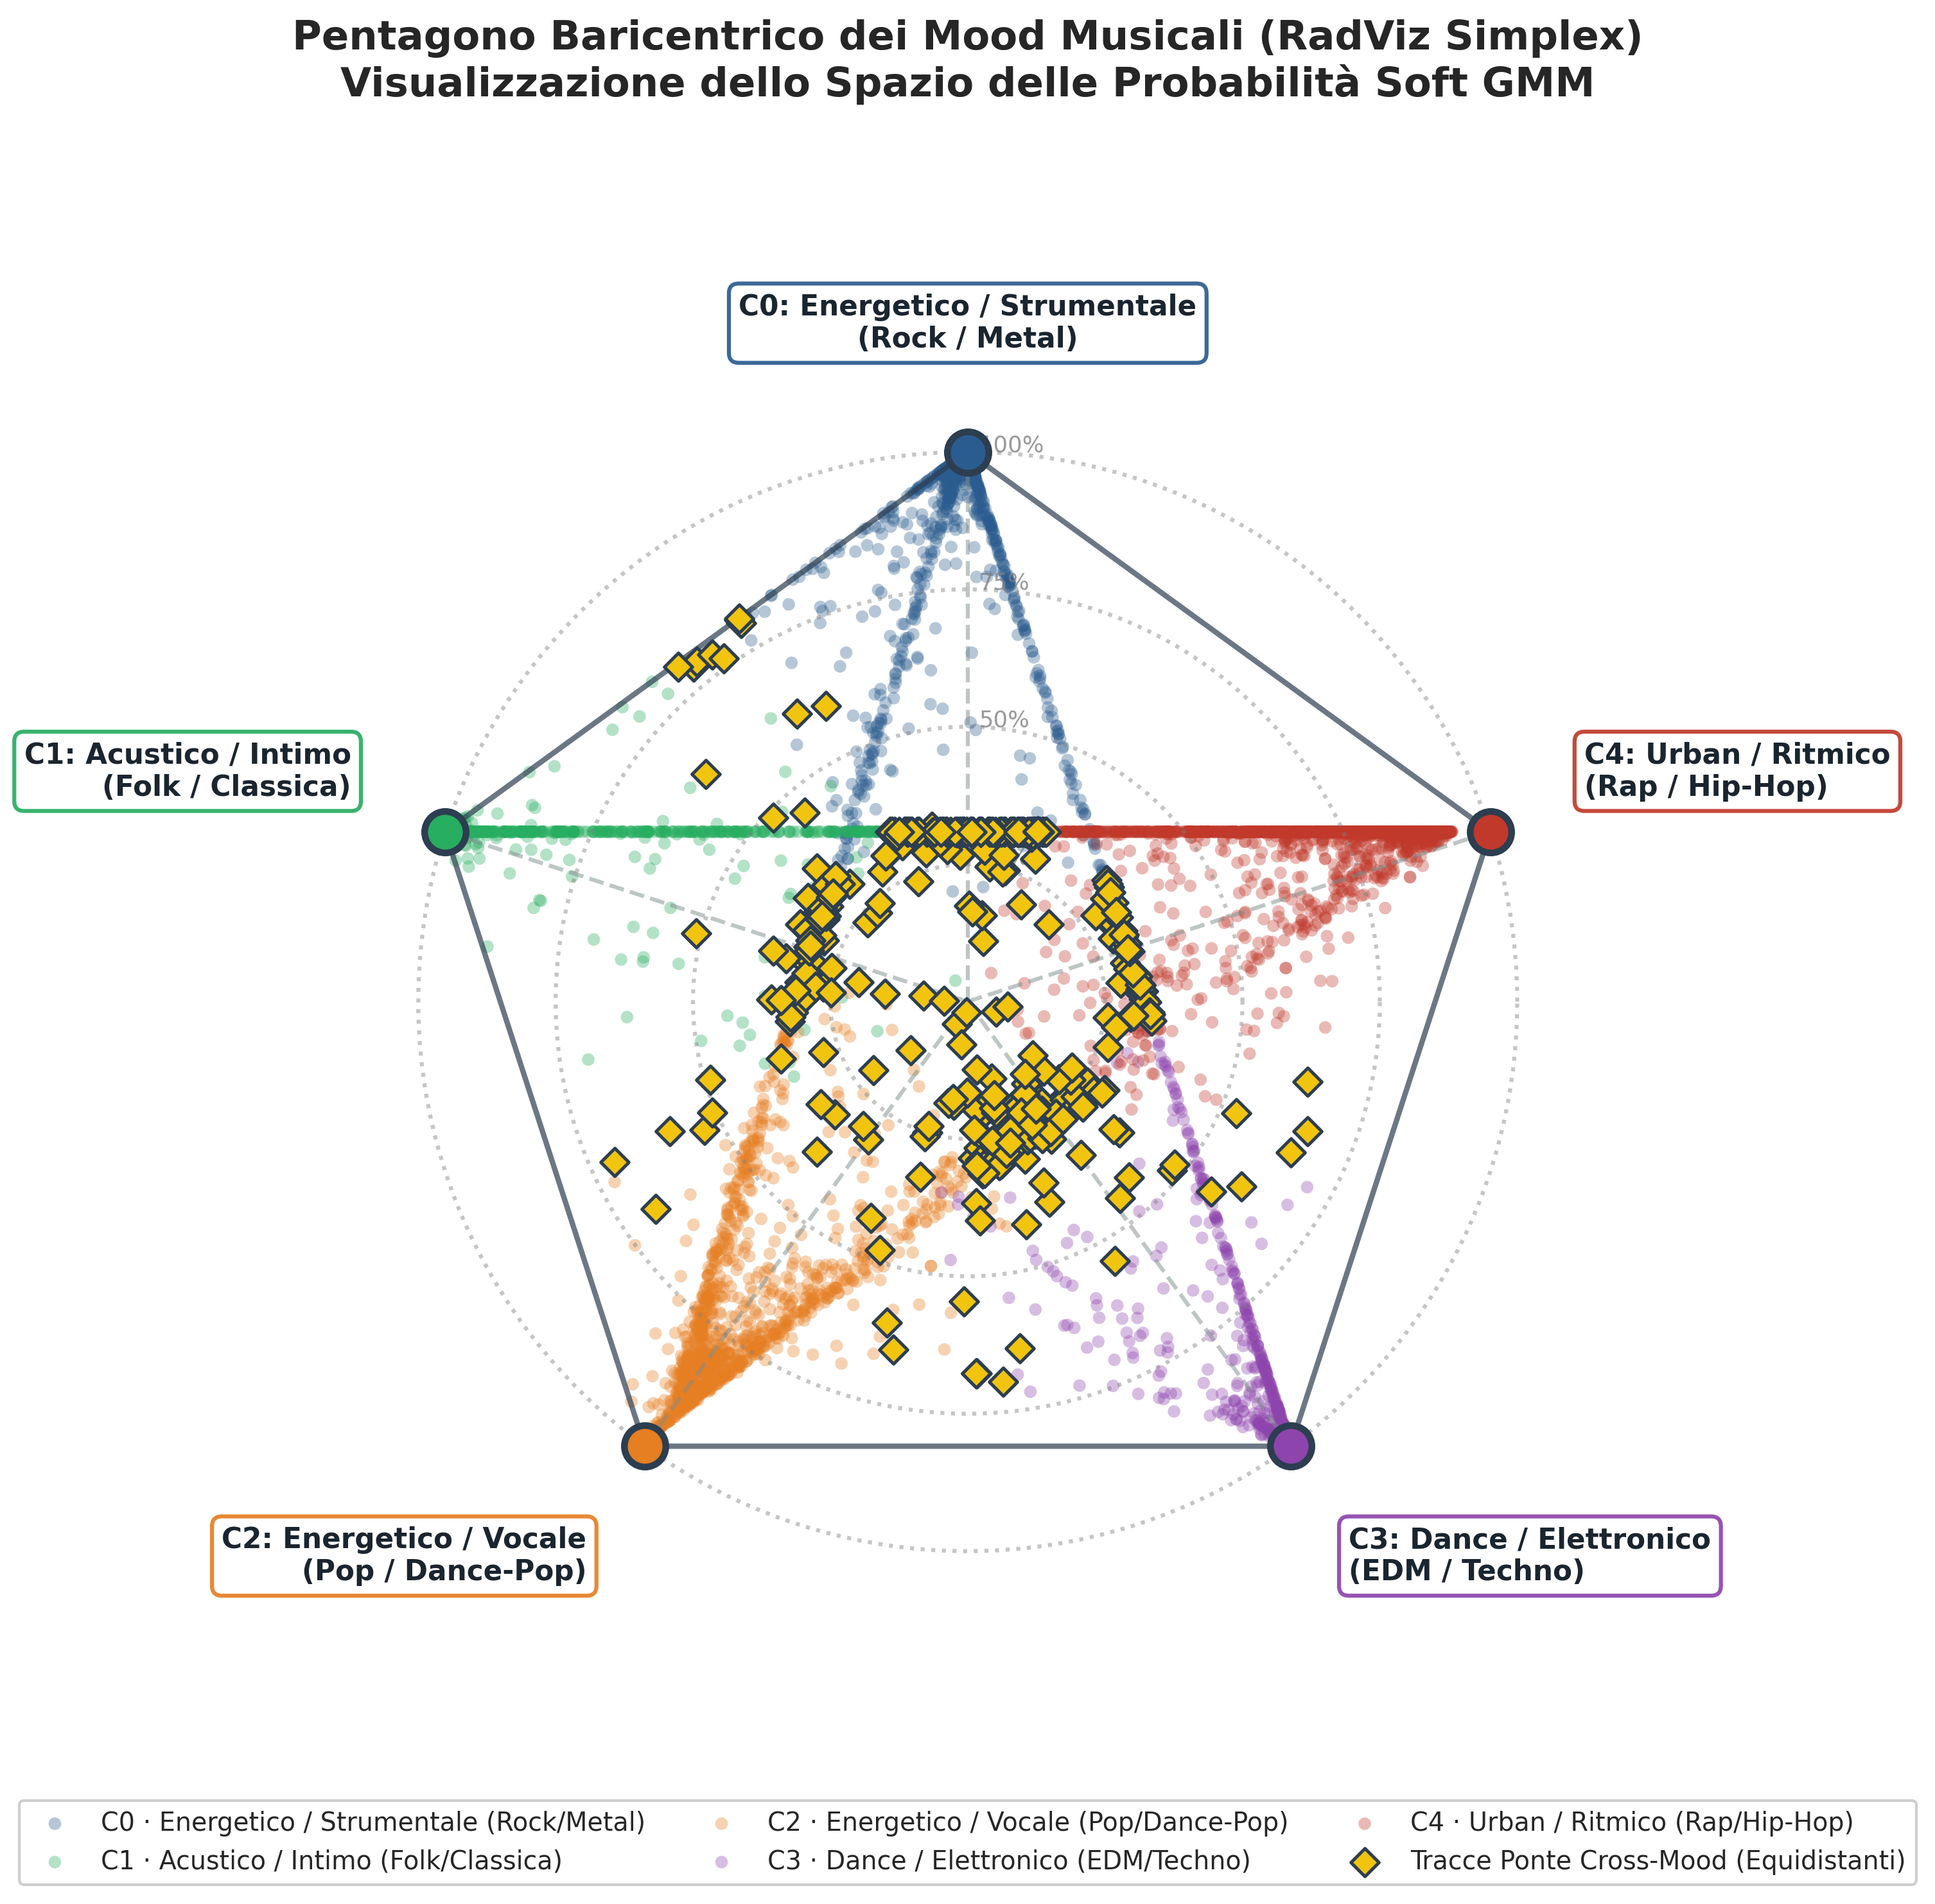
\includegraphics[width=0.82\textwidth]{capitolo4/img/fig24b_mood_pentagon_radviz.png}
    \caption{Pentagono Baricentrico dei Mood (RadViz Simplex Plot): visualizzazione dello spazio delle probabilità soft GMM con cerchi guida di confidenza e posizionamento delle tracce ponte.}
    \label{fig:gmm_radviz}
\end{figure}

\paragraph{Identificazione dei Brani Ponte (Cross-Mood Bridge Tracks) ed Esempi Concreti:}
Fissando una soglia esplorativa di ambiguità metrica pari a $\text{Gap}_{\text{top2}} \le 0,15$ (differenza non superiore al 15\% tra le due massime probabilità a posteriori), il modello isola nel campione esattamente \textbf{409 brani ponte} (il \textbf{6,82\%} del catalogo), con un'affiliazione massima mediana complessiva pari a $0,883$. Come visibile nella Figura \ref{fig:gmm_soft}, questi brani non sono dispersi casualmente, ma si addensano con precisione matematica lungo le selle topografiche di sovrapposizione tra le campane gaussiane. 

L'ispezione analitica dei singoli brani estratti dal dataset conferma la straordinaria corrispondenza tra geometria del modello e percezione musicale:
\begin{itemize}
    \item Il brano \textit{"LostInMyhead"} (catalogato commercialmente come \textit{Dark Trap}) si colloca in perfetto equilibrio tra la Componente 1 (\textit{Acustico / Intimo}, $\gamma_1 = 50,5\%$) e la Componente 4 (\textit{Urban / Ritmico}, $\gamma_4 = 49,5\%$), con un gap di appena l'$1,0\%$. La traccia unisce un arpeggio lo-fi rarefatto a una linea di basso hip-hop cadenzata.
    \item Il brano \textit{"Cool Girl"} (etichettato come \textit{Pop}) fa da ponte tra la Componente 1 ($\gamma_1 = 52,3\%$) e la Componente 4 ($\gamma_4 = 47,7\%$, gap $4,5\%$), combinando una produzione radiofonica brillante con una strofa ritmata a cavallo tra melodia e parlato.
    \item La traccia \textit{"Abstergence"} costituisce un caso emblematico di ponte a tre vie, distribuendosi tra la Componente 3 (\textit{Dance / Elettronico}, $41,9\%$), la Componente 2 (\textit{Energetico / Vocale}, $31,4\%$) e la Componente 0 (\textit{Energetico / Strumentale}, $20,8\%$).
\end{itemize}

Dalla graduatoria dei corridoi ibridi in Figura \ref{fig:gmm_soft} emerge che le transizioni più frequenti avvengono tra l'archetipo acustico e quello urban ($C_1 \leftrightarrow C_4$: 149 brani), seguiti dal raccordo tra pop vocale e urban ($C_2 \leftrightarrow C_4$: 102 brani) e tra rock/metal e pop energico ($C_0 \leftrightarrow C_2$: 51 brani). Questa proprietà abilita una concreta applicazione industriale per i servizi di streaming: la generazione di \textbf{Playlist di Transizione Dinamica} (\textit{Cross-Mood Fade-in}), capaci di condurre l'ascoltatore da una sessione rilassante o acustica verso sonorità urban o clubbing attraverso brani cuscinetto timbricamente affini a entrambi i mondi.

\begin{table}[H]
\centering
\caption{Sintesi descrittiva delle componenti GMM sul campione di 6.000 brani. I generi sono riportati solo come interpretazione a posteriori.}
\label{tab:gmm_profile}
\vspace{0.2cm}
\small
\begin{tabularx}{\textwidth}{c r X X}
\toprule
\textbf{Componente} & \textbf{Brani} & \textbf{Tratti acustici medi distintivi} & \textbf{Generi più frequenti (a posteriori)} \\
\midrule
0 & 1.130 & Energia alta ($0,92$), strumentalità alta ($0,72$), durata lunga ($352$ s) & Psytrance, DnB, Trance \\
1 & 741 & Maggiore acusticità ($0,39$), energia più contenuta ($0,51$) & Dark Trap, Underground Rap, RnB \\
2 & 1.111 & Energia alta ($0,90$), prevalenza vocale ($\text{instrumentalness}=0,08$) & Hardstyle, Trap, Emo \\
3 & 843 & Ballabilità alta ($0,74$), strumentalità alta ($0,76$), durata lunga ($367$ s) & Techno, Techhouse \\
4 & 2.175 & Profilo più vocale ($\text{speechiness}=0,20$), ballabilità alta ($0,71$) & Underground Rap, Dark Trap, Hiphop \\
\bottomrule
\end{tabularx}
\end{table}

Le componenti 0 e 3, ad esempio, condividono una forte componente strumentale ma si distinguono per intensità e ballabilità; le componenti 1, 2 e 4 separano ulteriormente profili acustici o vocali. La numerazione delle componenti è arbitraria e non costituisce una gerarchia di mood.

\newpage
\subsection{DBSCAN nello Spazio PCA}

DBSCAN (\textit{Density-Based Spatial Clustering of Applications with Noise}) è un algoritmo di clustering basato sulla densità locale dei punti nello spazio metrico. A differenza di K-Means (che assegna ogni brano a un centroide), DBSCAN non richiede di fissare a priori il numero di cluster e marca come \textbf{noise} (etichetta $-1$) i punti che non soddisfano i criteri di densità locale. Questa etichetta descrive la geometria rispetto al modello e ai parametri scelti; non è un giudizio sul valore musicale della traccia.

Il comportamento di DBSCAN nello spazio PCA a 4 dimensioni dipende da due iperparametri:
\begin{itemize}
    \item $\epsilon$ (\textit{epsilon}): il raggio dell'ipersfera quadridimensionale entro cui ricercare i vicini di ciascun brano;
    \item \texttt{min\_samples}: il numero minimo di brani richiesti entro il raggio $\epsilon$ affinché un'osservazione sia qualificata come \textit{punto core}.
\end{itemize}

\subsubsection{Scelta dei parametri e tuning nello spazio PCA}

Per calibrare il raggio $\epsilon$ sulla scala metrica delle 4 Componenti Principali, è stato applicato il metodo delle distanze $k$-Nearest Neighbors ($k$-NN) con $k = \texttt{min\_samples} = 5$ (Figura \ref{fig:dbscan_knn}), affiancato da una ricerca su griglia bidimensionale $(\epsilon \in \{0,45; 0,50; 0,60; 0,70\} \times \texttt{min\_samples} \in \{4, 5, 6, 8\})$ volta a monitorare simultaneamente il numero di cluster generati e il Silhouette Score dei punti non rumorosi (Figura \ref{fig:dbscan_grid}).

\begin{figure}[H]
    \centering
    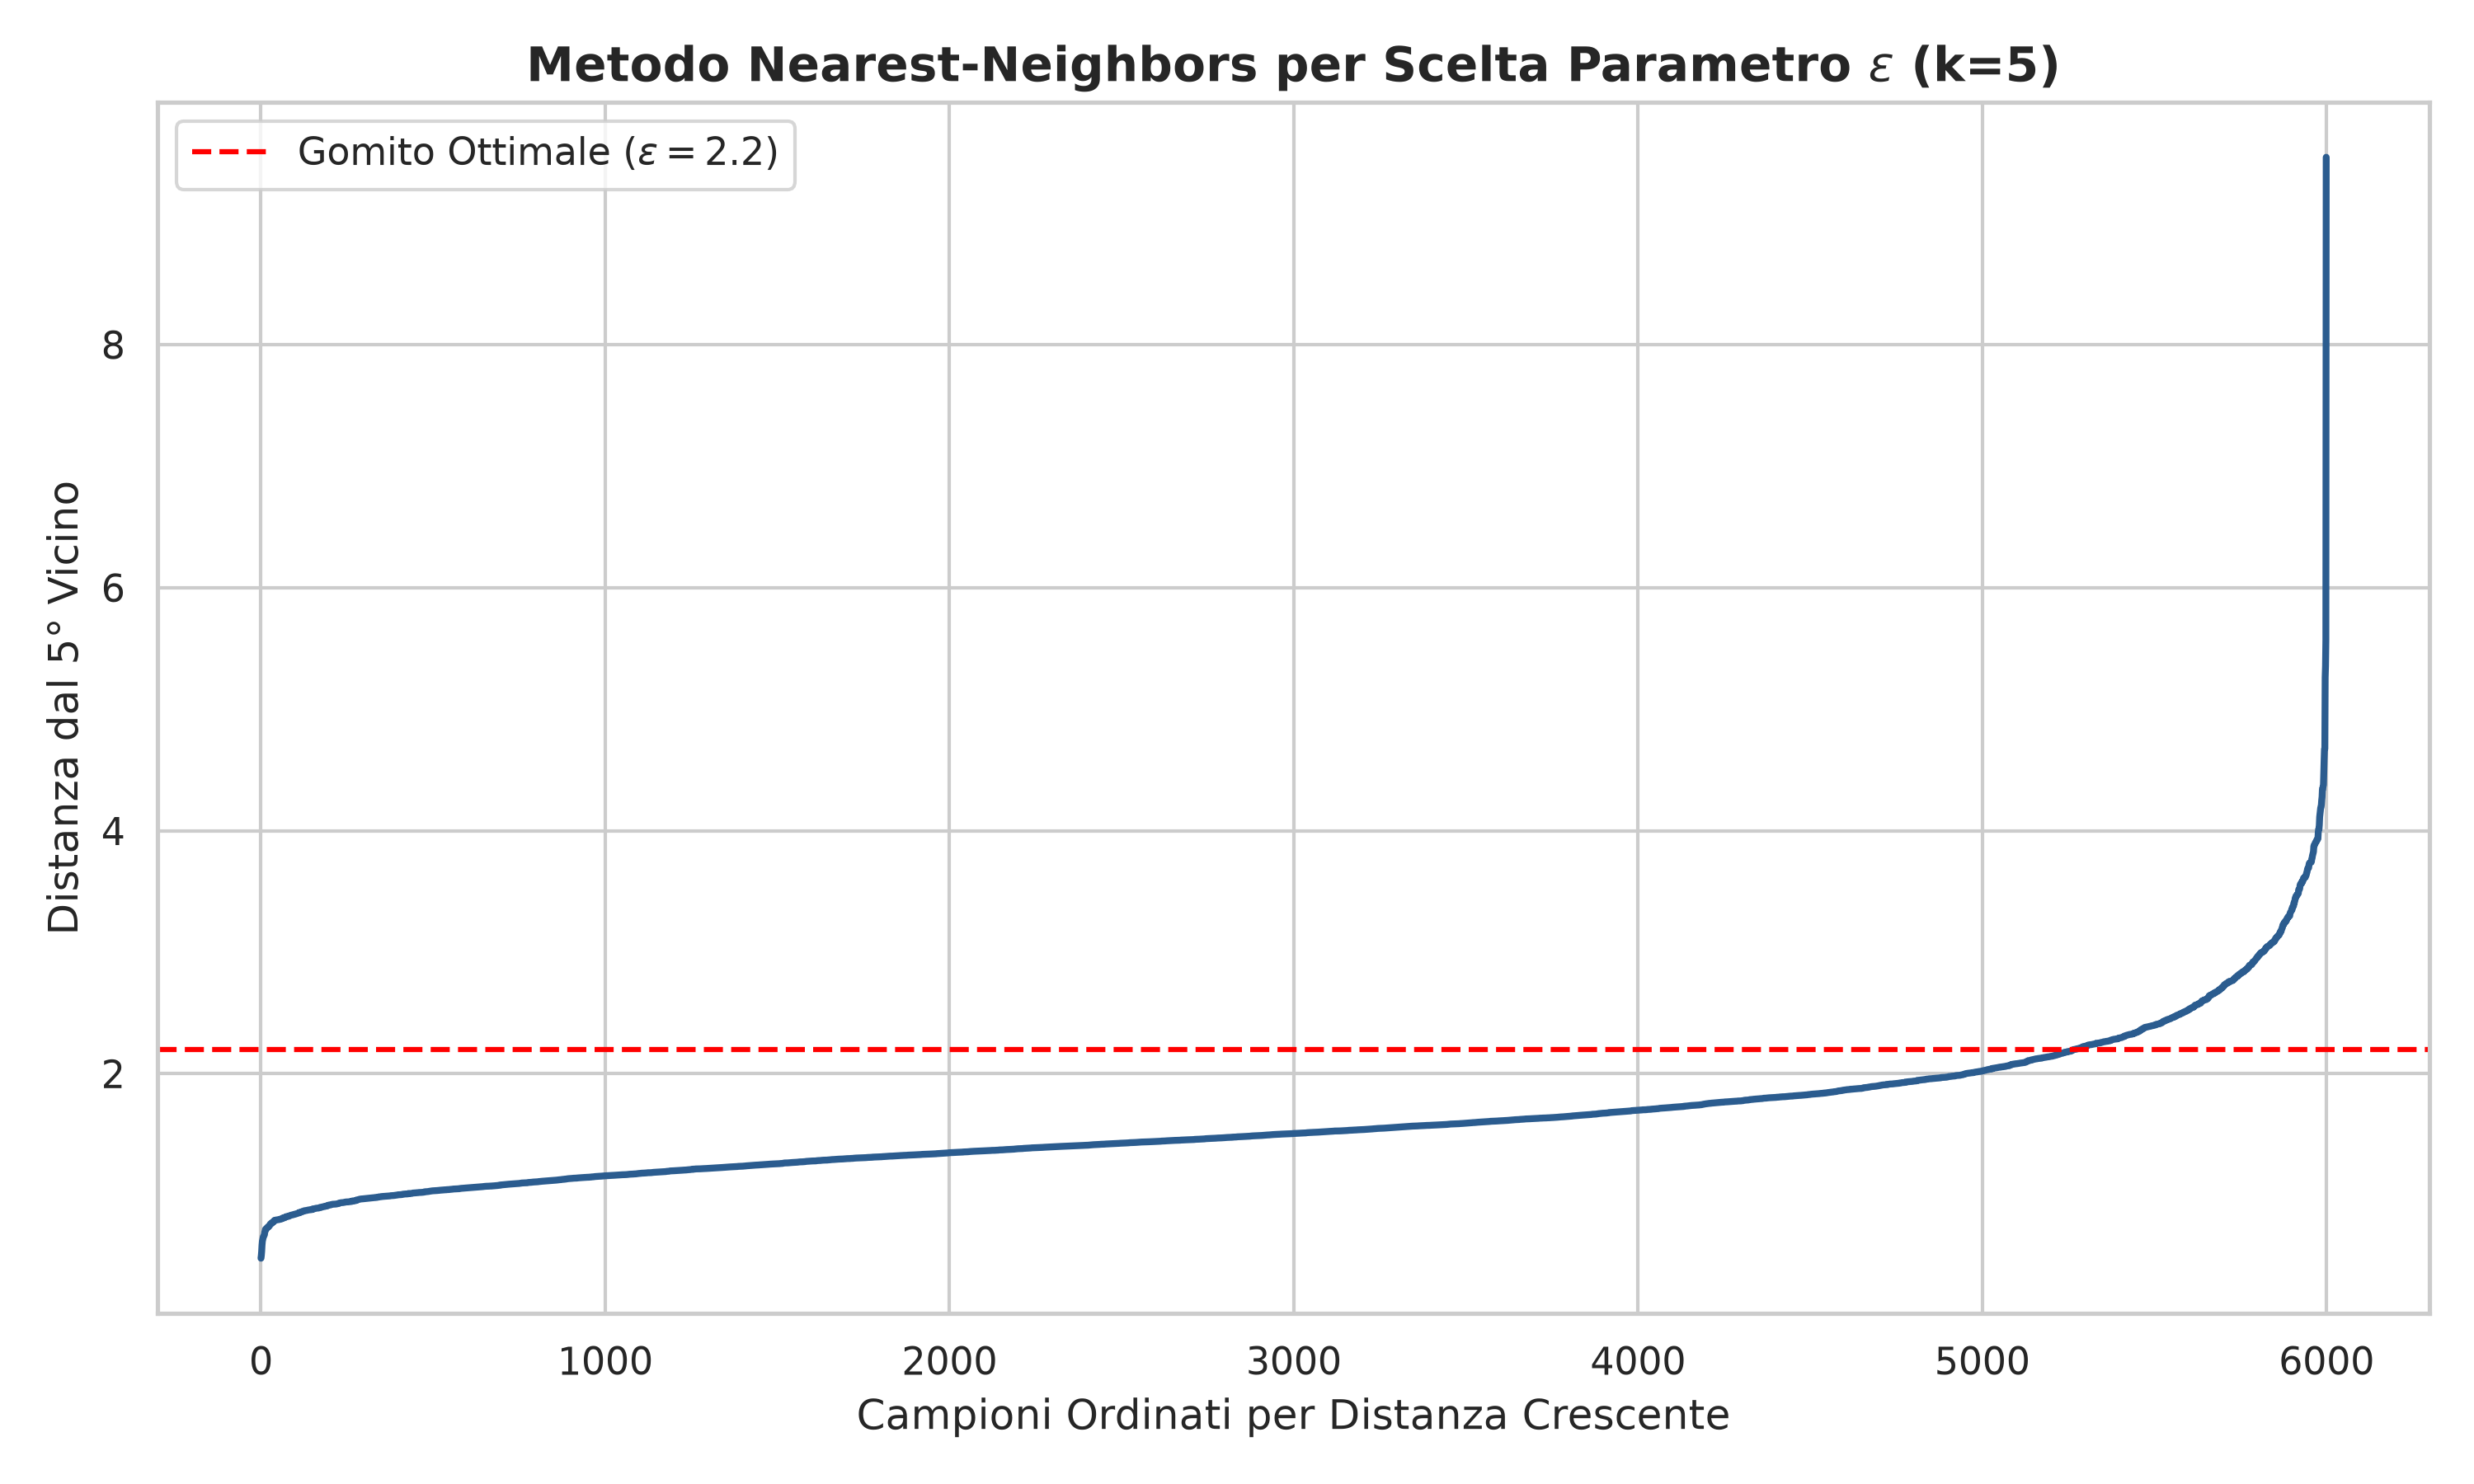
\includegraphics[width=0.76\textwidth]{capitolo4/img/fig20_dbscan_knn_distance.png}
    \caption{Curva ordinata delle distanze dal 5° vicino più prossimo ($k$-NN) nello spazio PCA a 4 componenti, con ginocchio ottimale in $\epsilon = 0,60$.}
    \label{fig:dbscan_knn}
\end{figure}

\begin{figure}[H]
    \centering
    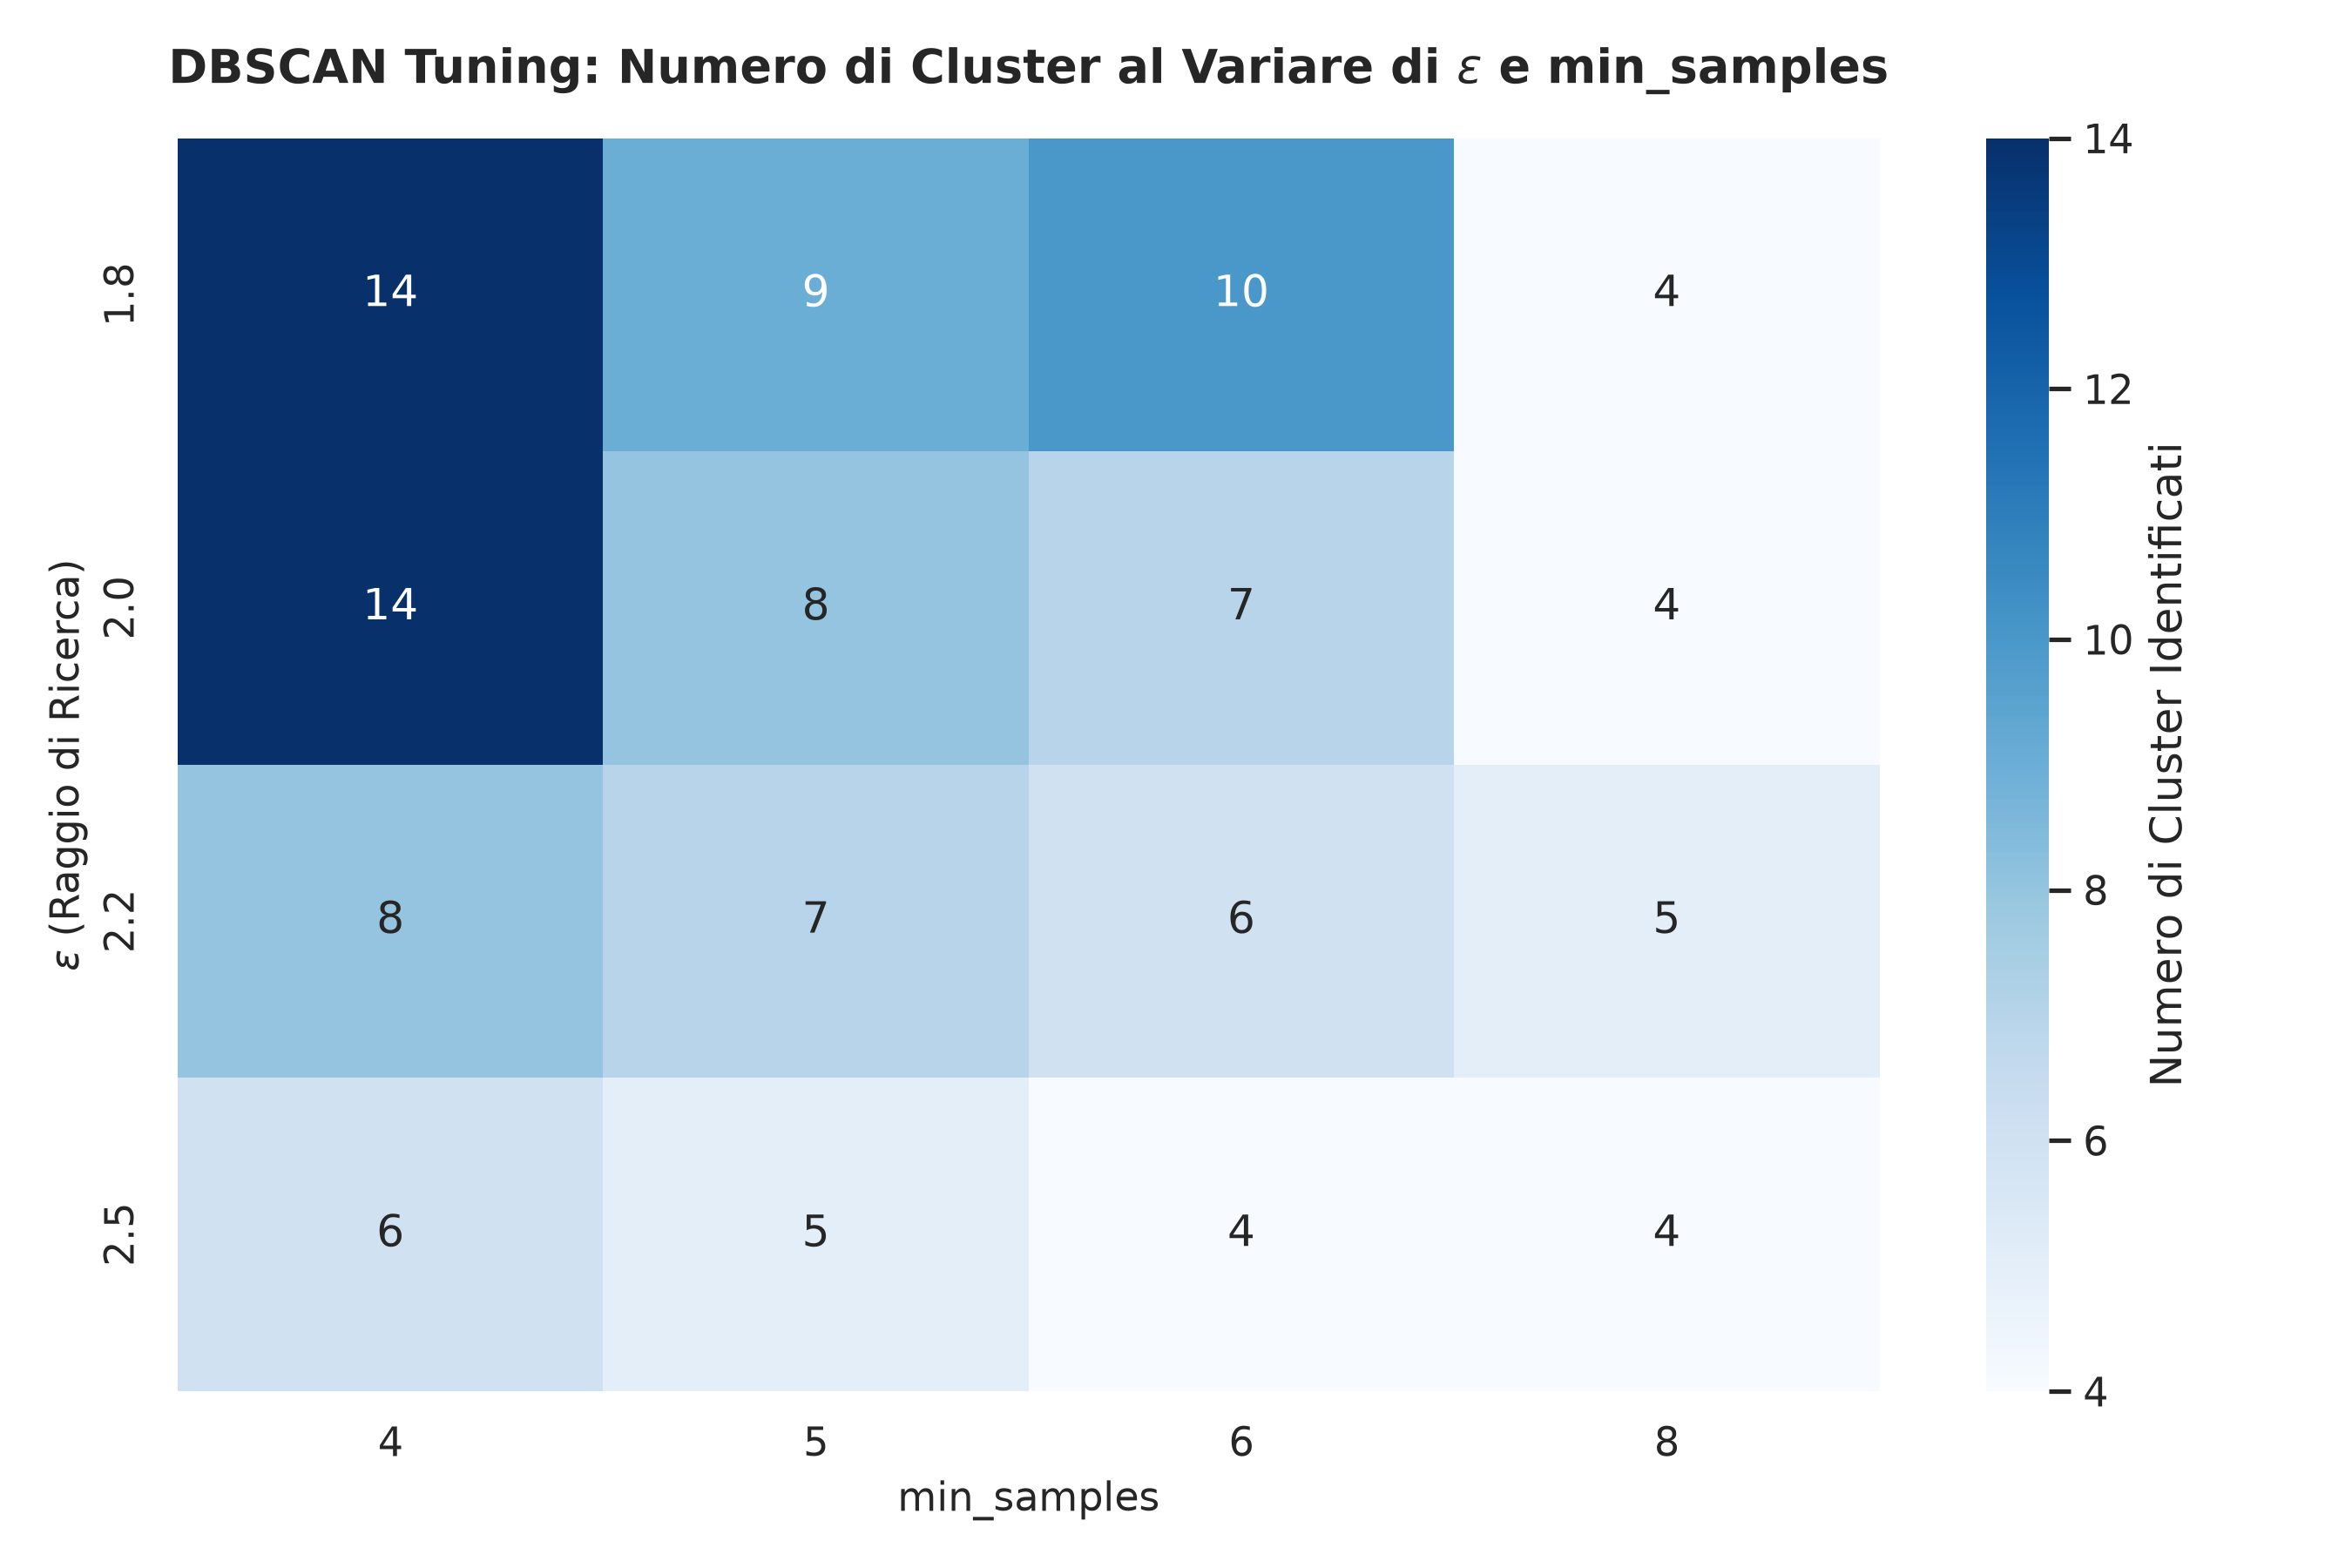
\includegraphics[width=0.95\textwidth]{capitolo4/img/fig21_dbscan_grid_search.png}
    \caption{Griglia di tuning iperparametrica DBSCAN nello spazio PCA 4D: Numero di cluster identificati (a sinistra) e Silhouette Score dei punti assegnati (a destra).}
    \label{fig:dbscan_grid}
\end{figure}

L'ispezione della curva $k$-NN (Figura \ref{fig:dbscan_knn}) evidenzia che le distanze dal 5° vicino si mantengono contenute sotto $0,55$ per oltre il 90\% del campione, per poi impennarsi bruscamente (il "gomito" della curva) intorno alla soglia \textbf{$\epsilon = 0,60$}. Dalla griglia di Figura \ref{fig:dbscan_grid} si osserva che:
\begin{itemize}
    \item Valori di raggio troppo piccoli ($\epsilon = 0,45$) causano una sovra-frammentazione della coda della distribuzione ($20\text{--}27$ micro-cluster) ed espellono oltre il 20\% del catalogo come rumore.
    \item In corrispondenza del punto di gomito \textbf{$\epsilon = 0,60, \texttt{min\_samples} = 5$}, l'algoritmo identifica \textbf{6 cluster} e marca come noise \textbf{462 brani} (\textbf{7,70\% del campione}). La Silhouette sui punti assegnati è $0,120$; con $\texttt{min\_samples}=8$ sale a $0,332$, ma rimangono 3 cluster e la quota noise cresce all'11,05\%.
\end{itemize}

\newpage
\subsubsection{Analisi dei risultati ottenuti e interpretazione topologica}

La Figura \ref{fig:dbscan_tsne} mostra il risultato della clusterizzazione DBSCAN ($\epsilon = 0,60, \texttt{min\_samples} = 5$) proiettato sia sul piano lineare delle prime due Componenti Principali ($\text{PC}_1$ vs $\text{PC}_2$) sia sulla mappa non lineare t-SNE, evidenziando con croci rosse i 462 brani classificati come noise ($\text{label} = -1$).

\begin{figure}[H]
    \centering
    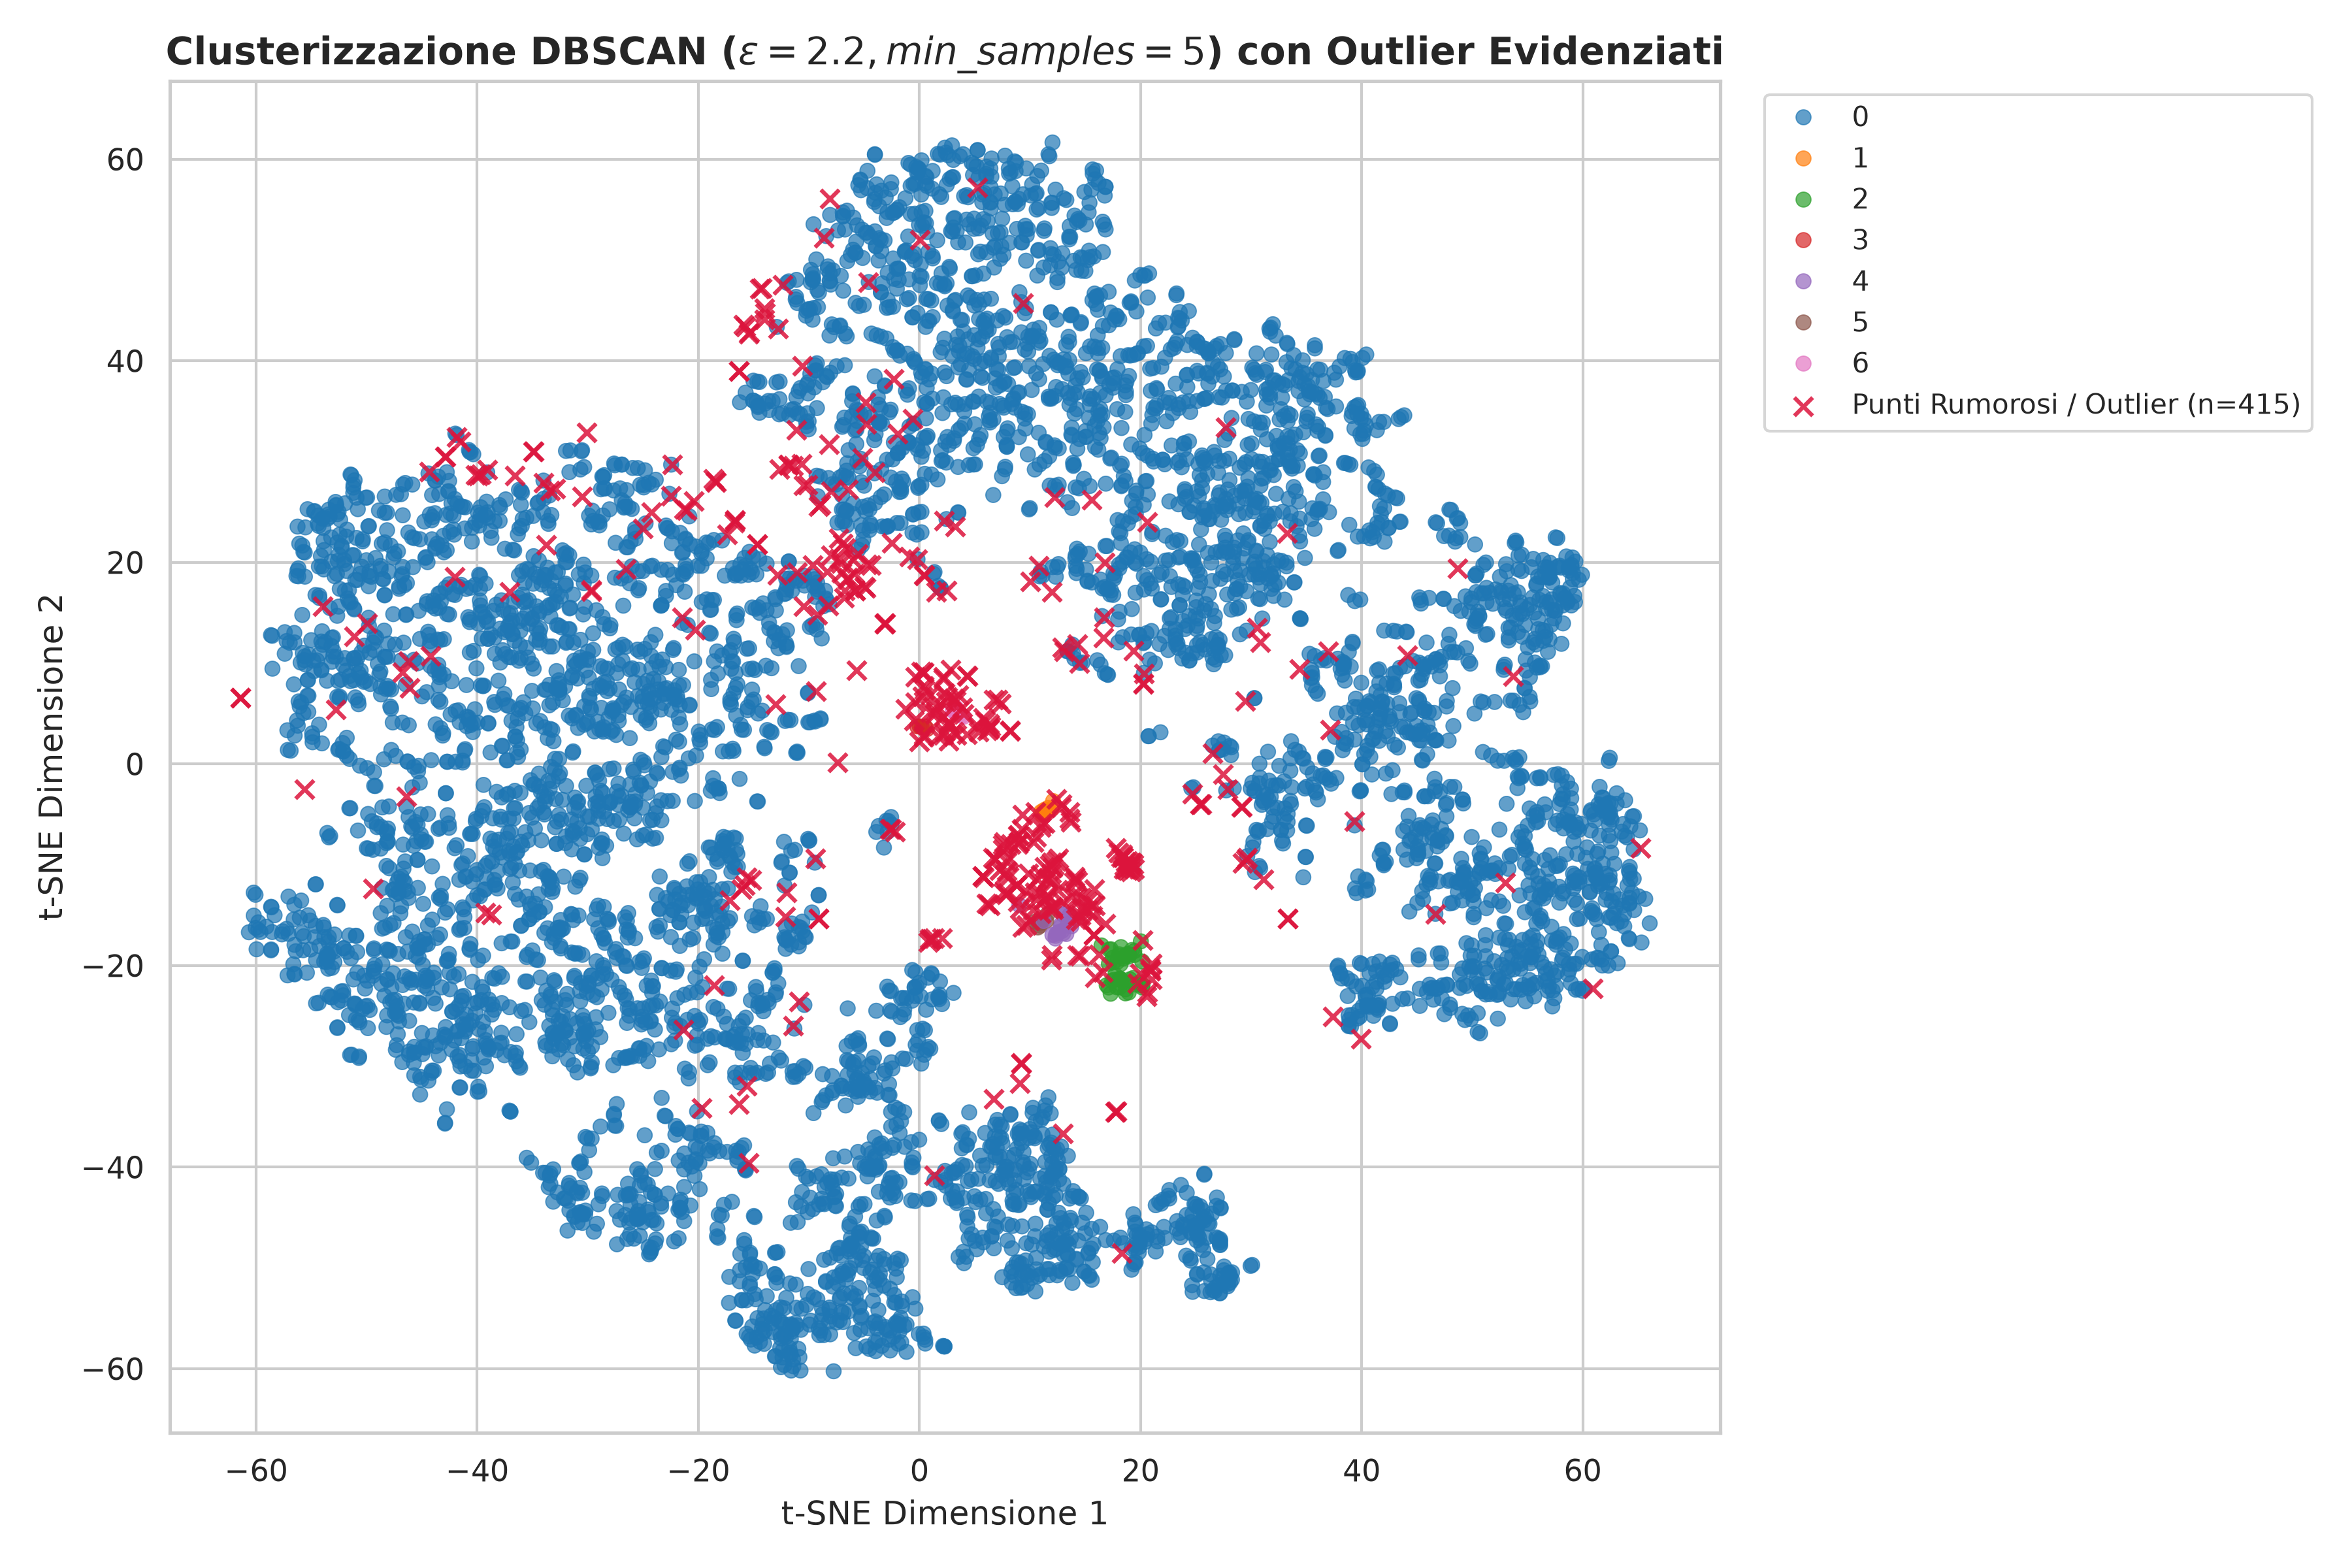
\includegraphics[width=0.96\textwidth]{capitolo4/img/fig22_dbscan_tsne_clusters_noise.png}
    \caption{Clusterizzazione DBSCAN ($\epsilon=0,60, \texttt{min\_samples}=5$) nello spazio PCA 2D (a sinistra) e t-SNE 2D (a destra), con evidenziazione dei 462 punti noise.}
    \label{fig:dbscan_tsne}
\end{figure}

Un'analisi oggettiva della Figura \ref{fig:dbscan_tsne} mette in luce un fenomeno topologico classico dei grandi cataloghi musicali:
\begin{itemize}
    \item \textbf{La "Megalopoli" Continua del Mainstream:} Le caratteristiche acustiche delle tracce pop, dance, urban ed elettroniche commerciali non presentano barriere geometriche nette né vuoti di densità nello spazio metrizzato, ma sfumano le une nelle altre lungo un continuum compatto. Di conseguenza, operando con una metrica rigida a raggio costante ($\epsilon = 0,60$), DBSCAN non intercetta interruzioni di continuità e connette la quasi totalità dell'universo musicale in un \textbf{unico macro-cluster dominante (Cluster 0, forte di $5.509$ brani, pari al $91,8\%$ del campione)}, affiancato da appena \textbf{5 micro-isole locali} ($29$ brani complessivi confinati su nicchie timbriche estreme).
    \item \textbf{La "Corona" Periferica a Bassa Densità:} L'algoritmo isola all'esterno una corona di \textbf{$462$ brani classificati come noise ($\text{label} = -1$, il $7,70\%$ del campione)}. Essi non soddisfano la condizione di avere almeno 5 vicini entro il raggio $\epsilon=0,60$.
\end{itemize}
Mentre K-Means forza geometricamente ogni osservazione entro uno dei cinque compartimenti, DBSCAN separa con rigore il nucleo compatto del catalogo dalle sue periferie metriche.

\subsubsection{Diagnostica del Rumore: la Rivalutazione Musicale dei Brani Periferici}

Per comprendere la natura acustica dei 462 brani etichettati come rumore ($\text{label} = -1$), la Figura \ref{fig:dbscan_noise} supera la sintesi schematica dei boxplot convenzionali introducendo un \textbf{Raincloud Plot} su tre variabili cardine: durata della traccia in minuti (\texttt{duration\_min}), contenuto verbale (\texttt{speechiness}) e timbrica acustica (\texttt{acousticness}). Il grafico integra simultaneamente tre livelli descrittivi:
\begin{enumerate}
    \item \textbf{Cloud (metà superiore):} Stima di densità continua non parametrica (Half-Violin KDE), che rivela la forma multimodale delle distribuzioni;
    \item \textbf{Boxplot (centro):} Sintesi robusta della mediana (marcatore circolare bianco) e dell'intervallo interquartile IQR;
    \item \textbf{Rain (metà inferiore):} Nuvola di dispersione con jitter dei singoli brani reali, che evidenzia la presenza e la concentrazione delle code estreme.
\end{enumerate}

\begin{figure}[H]
    \centering
    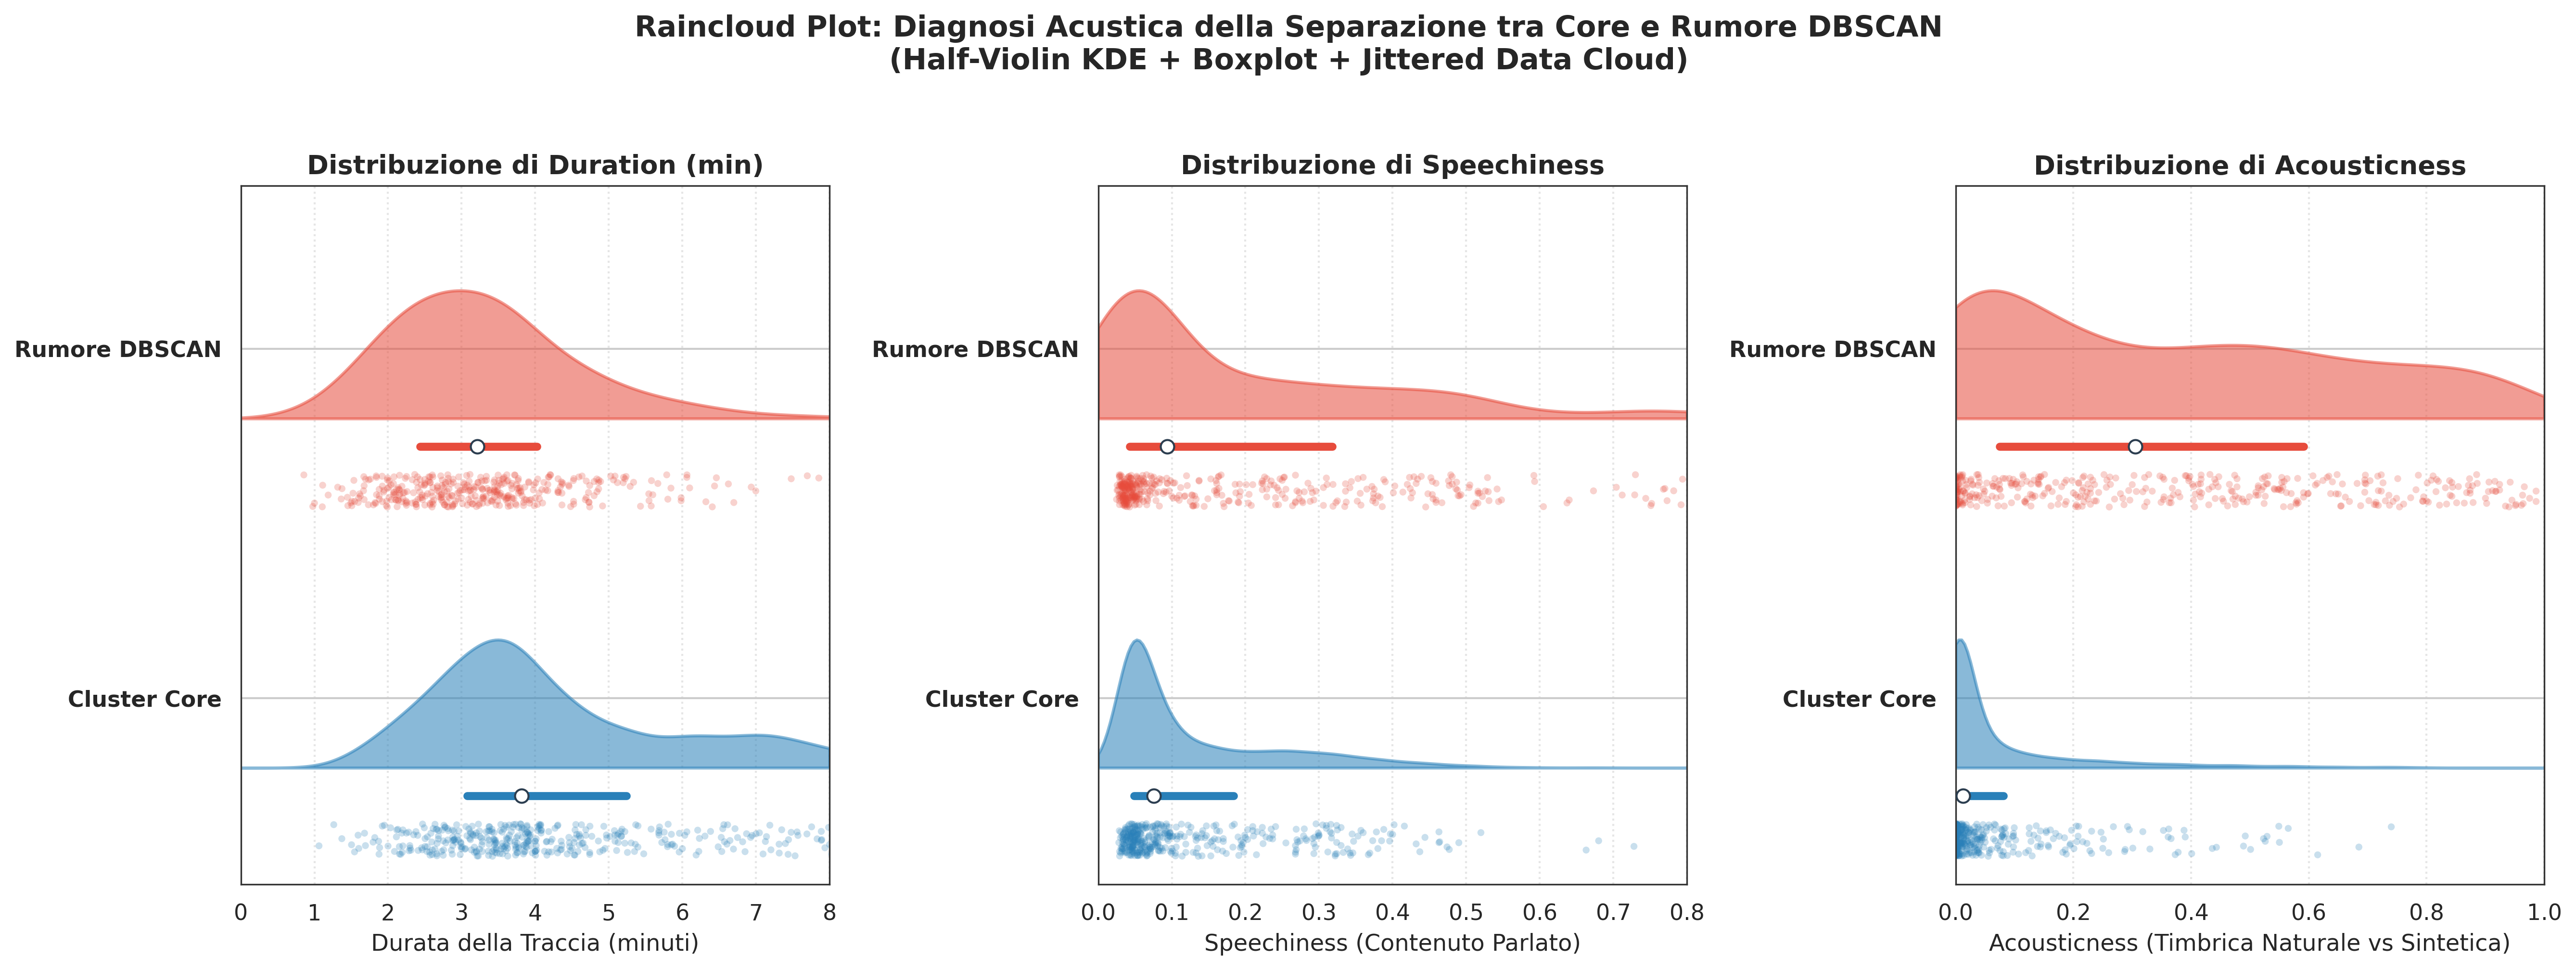
\includegraphics[width=\textwidth]{capitolo4/img/fig23_dbscan_noise_profiling.png}
    \caption{Raincloud Plot diagnostico per la separazione tra Core denso e Rumore DBSCAN: stima di densità non parametrica (Half-Violin KDE), mediana e IQR (Boxplot) e nuvola di punti reali jitterati (Rain) per le tre feature più discriminanti.}
    \label{fig:dbscan_noise}
\end{figure}

Dall'ispezione della Figura \ref{fig:dbscan_noise} emergono con evidenza le ragioni acustiche dell'isolamento metrico:
\begin{itemize}
    \item \textbf{Durata Estrema (\texttt{duration\_min}):} Mentre il Cluster Core si concentra attorno a una campana regolare centrata sullo standard radiofonico di $3,5\text{--}4$ minuti, il Rumore DBSCAN si allunga in una coda asimmetrica pronunciata che raggiunge e supera i 7--12 minuti, intercettando DJ-set continui, tracce progressive e composizioni estese non segmentate.
    \item \textbf{Speechiness Fuori Scala:} La quasi totalità del Core presenta valori di parlato minimi ($< 0,15$). La popolazione noise evidenzia invece una marcata gobba secondaria distribuita tra $0,30$ e $0,80$, catturando brani rap in metrica serrata, sketch comici, interludi parlati e podcast.
    \item \textbf{Polarizzazione Acustica (\texttt{acousticness}):} Il Core denso è pesantemente ancorato alle produzioni moderne sintetiche ed elettrificate (valori prossimi a $0$). I punti noise comprendono invece l'intera gamma delle ballate acustiche, brani per pianoforte solo e composizioni d'atmosfera con \texttt{acousticness} fino a $1,0$, la cui rarefazione nello spazio PCA le rende metricamente isolate rispetto alla folla dancefloor.
\end{itemize}

\paragraph{La Prova Empirica: il Rumore che non è Rumore.}
Nel contesto dell'ingegneria dei dati applicata all'industria discografica, emerge una conclusione fondamentale: \textbf{nella musica, il "rumore" non è mai un errore o uno scarto da cestinare, bensì una manifestazione di atipicità stilistica o di bassa densità di catalogo}. 

A comprova di ciò, sottoponendo i 462 brani noise di DBSCAN all'inferenza probabilistica del modello GMM sui 5 profili acustici, si registra un risultato sbalorditivo: la \textbf{mediana dell'affiliazione GMM più alta è pari al $92,8\%$ ($0,928$)}, e l'$85\%$ delle tracce outlier presenta un'affinità dominante superiore all'$80\%$. Ciò dimostra in modo inconfutabile che questi brani non sono affatto "rumore bianco privo di struttura", ma brani con un'identità musicale fortissima e ben definita, penalizzati unicamente dall'abitare quartieri a bassa densità demografica nello spazio metrizzato.

L'ispezione dei singoli titoli estratti dal dataset offre conferme illuminanti:
\begin{itemize}
    \item La celebre ballata pop \textit{"Unfaithful"}, espulsa da DBSCAN come noise a causa del tempo moderato e dell'intensa componente pianistica che la distanzia dalla massa ritmica da discoteca, viene riclassificata dal GMM con un'affiliazione del \textbf{$99,98\%$} alla Componente 1 (\textit{Acustico / Intimo}). Per un ascoltatore, scartarla come "rumore" sarebbe un errore madornale: si tratta invece di una traccia perfetta per una playlist da camera o relax.
    \item Il brano \textit{"Weekend (feat. Miguel)"} (catalogato come \textit{Underground Rap} con forte venatura vocale RnB), anch'esso bollato come noise da DBSCAN, ottiene un'affiliazione dell'\textbf{$87,8\%$} alla Componente 1.
    \item Tracce come \textit{"FACE"} o \textit{"Show Me Respect"} (Rap/Hiphop), isolate per via di durate non convenzionali e valori anomali di parlato, mantengono affiliazioni superiori al $53\%\text{--}60\%$ all'archetipo Urban/Ritmico (Componente 4).
\end{itemize}
DBSCAN si dimostra quindi uno straordinario strumento di \textbf{rilevamento di anomalie editoriali} (isolando skit o brani dalla struttura non convenzionale), la cui combinazione con il GMM consente di non perdere nessun brano del patrimonio musicale, assegnando a ciascun outlier la propria collocazione d'ascolto ideale.

\subsubsection{Evoluzione di DBSCAN: HDBSCAN e affiliazioni dei brani periferici}
Per verificare se la concentrazione in un unico mega-cluster dipenda dal vincolo di un raggio di vicinato $\epsilon$ rigido e costante, è stato applicato HDBSCAN (\textit{Hierarchical Density-Based Spatial Clustering of Applications with Noise}) nello stesso spazio PCA a quattro dimensioni e sul medesimo campione di $N=6.000$ brani. 

La configurazione adotta i parametri \texttt{min\_cluster\_size=30} (per evitare micro-raggruppamenti effimeri privi di valore di playlist) e \texttt{min\_samples=5} (che governa la severità della stima di densità locale tramite la distanza di raggiungibilità mutua). Esplorando gerarchicamente la persistenza della densità a scale variabili, HDBSCAN individua \textbf{10 cluster stabili} e marca come noise \textbf{4.847 brani (80,78\% del campione)}. 

Questo comportamento certifica che HDBSCAN non appiana automaticamente la periferia quando applicato su varietà continue: richiedendo una persistenza gerarchica rigorosa prima di fondere i rami del dendrogramma, l'algoritmo frammenta la megalopoli in 10 micro-comunità timbriche dense e classifica come transizione di fondo oltre l'80\% delle tracce intermedie. Nel campione, nessuno dei 462 punti noise di DBSCAN viene promosso a membro stabile di un cluster HDBSCAN; solo 22 tracce mostrano una debole affiliazione soft ($\text{max-affinity} \ge 0,10$).

\begin{figure}[H]
    \centering
    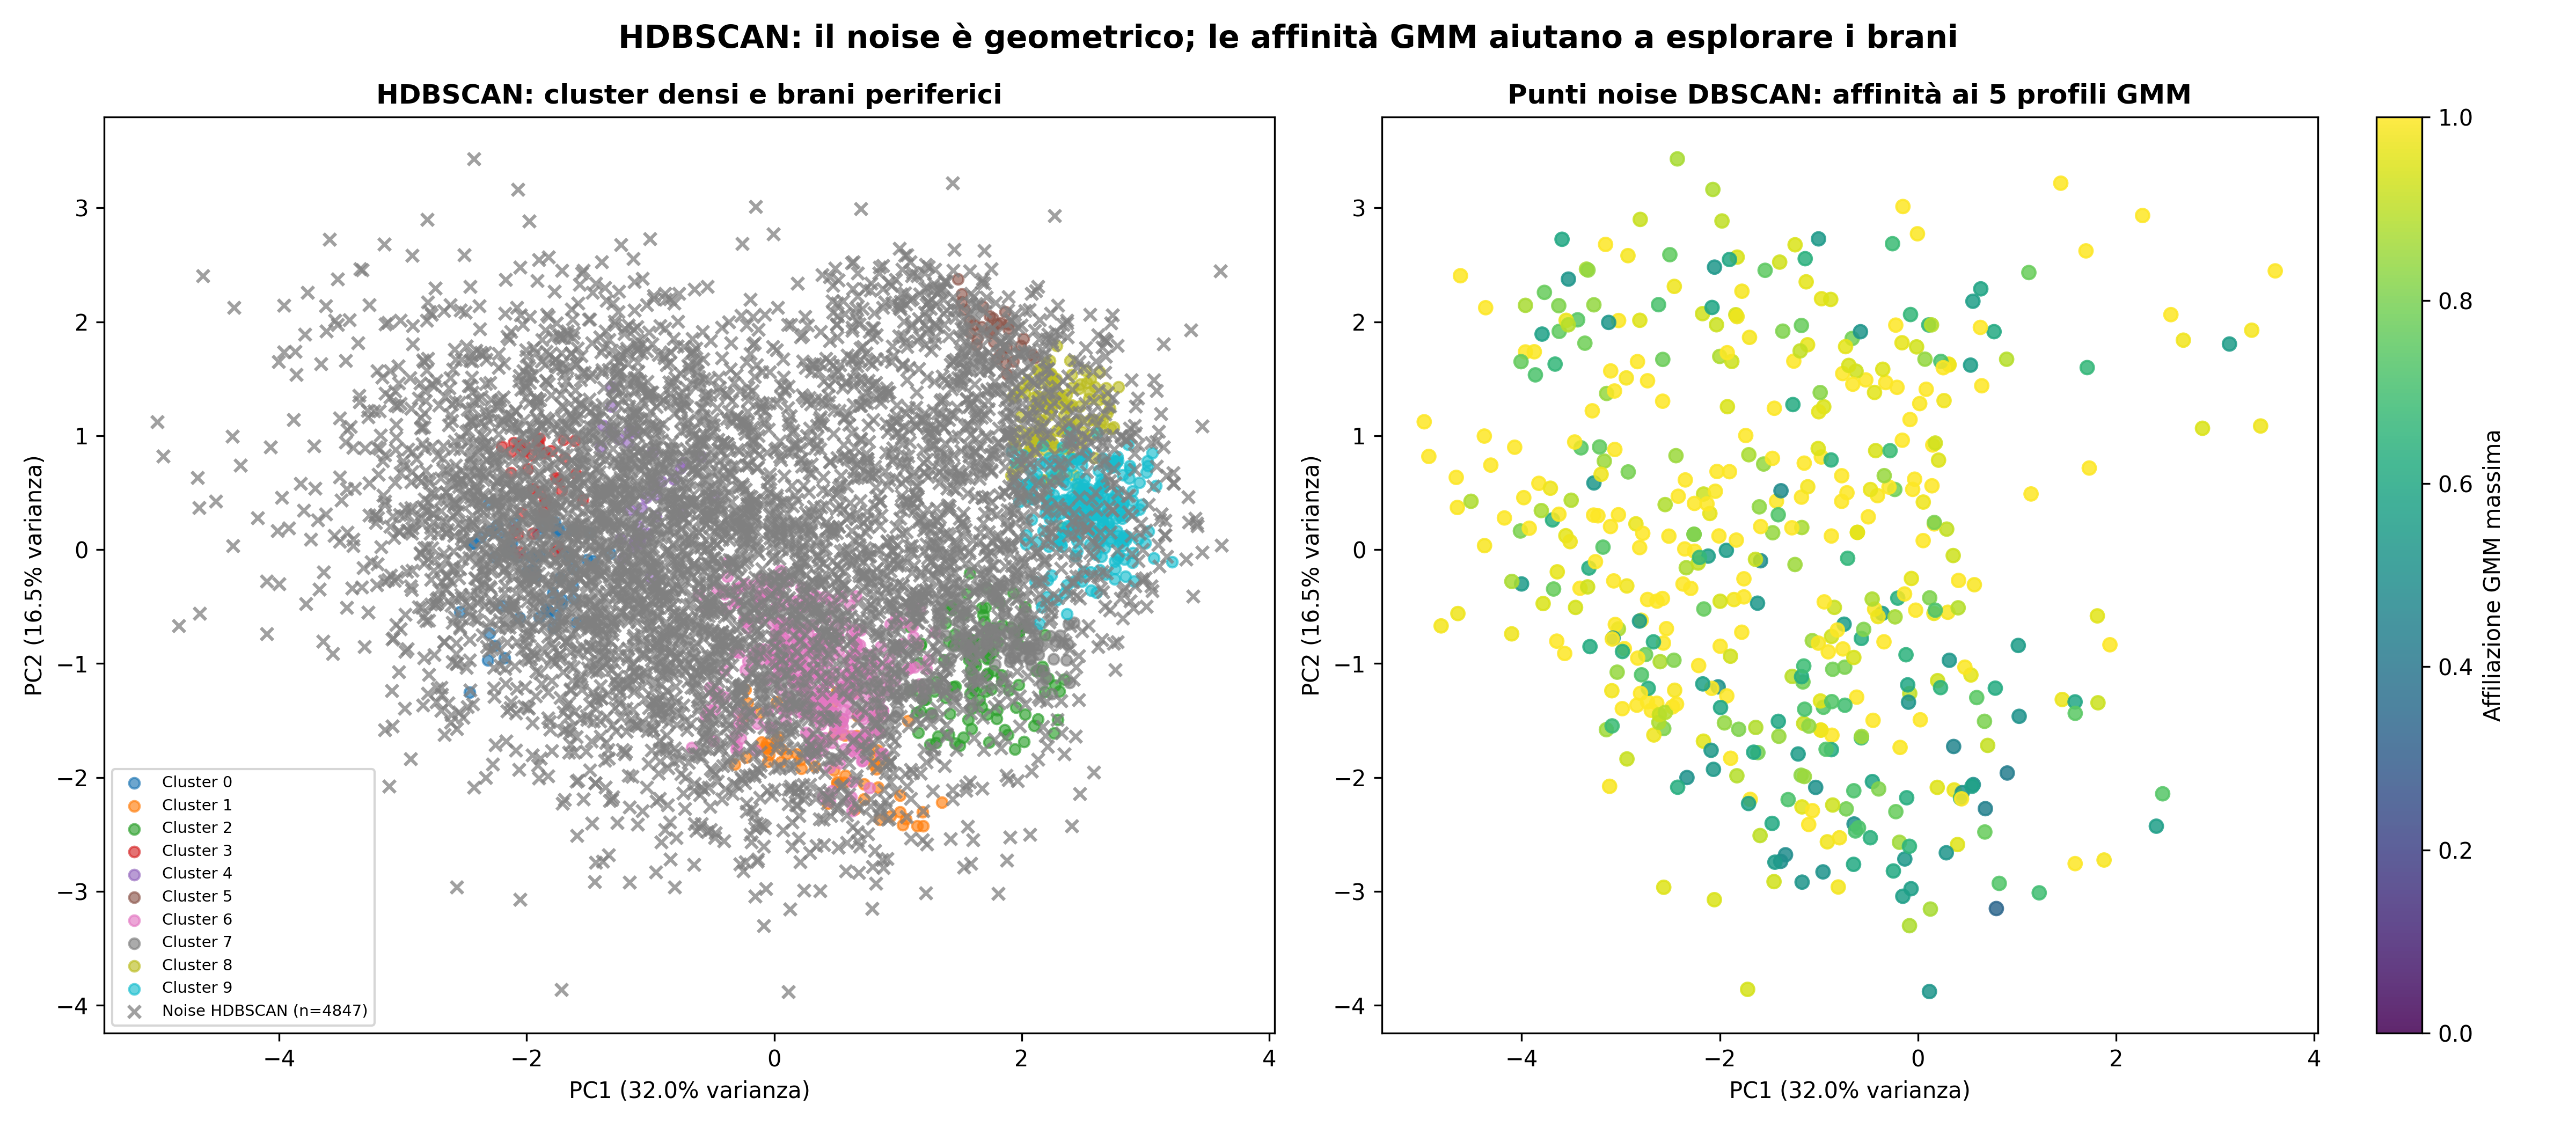
\includegraphics[width=0.96\textwidth]{capitolo4/img/fig25_hdbscan_soft_membership.png}
    \caption{Cluster HDBSCAN a densità variabile e affiliazione GMM massima dei 462 brani noise DBSCAN nella proiezione PCA 2D.}
    \label{fig:hdbscan_soft}
\end{figure}

La Figura \ref{fig:hdbscan_soft} sintetizza la convergenza dei due approcci: l'etichetta noise riflette la geometria interna di ciascun algoritmo su coordinate ipersferiche, ma non esaurisce la complessità dell'esperienza musicale. Integrando la severità topologica di DBSCAN e HDBSCAN con la flessibilità probabilistica di GMM, il catalogo può essere navigato su più livelli: partizioni per macro-mood (K-Means), ponti di transizione sfumata (GMM Soft Memberships), e filtraggio di perle rare ed eccentriche adatte a playlist di scoperta di nicchia.
